\documentclass[vi]{uet-awesome-thesis} % use [vi] for vietnamese
\setlength{\parindent}{0pt}
\usepackage{blindtext}
\usepackage{graphicx}
\usepackage{array}
\setcounter{tocdepth}{3}


% \title{This is title of the thesis}
% \author{Trần Thế Phong}
% \major{Công Nghệ Thông Tin}
% \advisor{Prof. Lê Thanh Hà}
% \university{University of Engineering and Technology}
% \universitycity{Hanoi}
% \degreeyear{2022}

% \renewcommand{\glsmcols}{2}
\setglossarystyle{mcolindex}

\newacronym{wsn}{WSN}{wireless sensor network}
\newacronym{wrsn}{WRSN}{wireless rechargeable sensor network}
\newacronym{qos}{QoS}{Quality of Service}
\newacronym{ia}{IA}{intelligent agent}
\newacronym{rl}{RL}{reinforcement learning}
\newacronym{dl}{DL}{deep learning}
\newacronym{mdp}{MDP}{Markov decision process}



\newglossary[nlg]{notation}{not}{ntn}{Notation}

\newglossaryentry{not:eth}{
    name=\ensuremath{\tilde{E}_{td}},
    description={energy requesting threshold},
    type=notation}
    
\newglossaryentry{not:bs}{
    name=\ensuremath{p_0},
    description={base station},
    type=notation}
    
\newglossaryentry{not:snset}{
    name=\ensuremath{\mathcal{P}},
    description={a set of deployed sensors},
    type=notation}

\newglossaryentry{not:num:sn}{
    name=\ensuremath{n},
    description={number of deployed sensors},
    type=notation}
    
\newglossaryentry{not:sn}{
    name=\ensuremath{p},
    description={a sensor},
    type=notation}
    

% \makeglossaries 

\begin{document}
%%%%%%%%%%%%%%%%%%%%%%%%%%%%%%%%
%title 
%%%%%%%%%%%%%%%%%%%%%%%%%%%%%%%%
% \maketitle
% 
% \makesidecover

% \authorship

% \approval

% called by main.tex


% This is the cover page rectangle frame
\begin{tikzpicture}[overlay,remember picture]
\draw [line width=1.5mm]
    ($ (current page.north west) + (1.6cm,-1.6cm) $)
    rectangle
    ($ (current page.south east) + (-1.0cm,1.0cm) $);
\draw [line width=0.5mm]
    ($ (current page.north west) + (1.8cm,-1.8cm) $)
    rectangle
    ($ (current page.south east) + (-1.2cm,1.2cm) $);
\end{tikzpicture}


\thispagestyle{empty}
\begin{center} \centering
    \textbf{ĐẠI HỌC CÔNG NGHỆ - ĐHQGHN}\\
    \textbf{KHOA CÔNG NGHỆ THÔNG TIN}\\
\end{center}

\begin{center}

\includegraphics[width = 3\linewidth, height = 5cm, keepaspectratio]{UET_logo.png}
\vspace{15 mm}
\begin{spacing}{1.0}
\textbf{\large {INT3234E 53 - Phân tích dữ liệu dự báo}}\\
\textbf{\large {Báo cáo tiểu luận cuối kì}}\\
\end{spacing}
\vspace{10 mm}

% This is a large blank space in the middle of the report
\begin{spacing}{2.0}
\textbf{\LARGE {PHÂN TÍCH DỰ ĐOÁN GIÁ BITCOIN SỬ DỤNG HỌC MÁY}}
\end{spacing}

\vspace{5 mm}

\begin{spacing}{0.8}
{\large {Bài báo gốc: Analysis of Bitcoin Price Prediction Using Machine Learning}}
\end{spacing}
\end{center}


\begin{center}
\begin{spacing}{0.5}
\textbf{\large {Hoàng Bảo An - 22024545}}\\
\textbf{\large {Lê Tuấn Kiệt - 22024546}}\\
% {\large {\priorstudies}}\\
\end{spacing}
\end{center}

\vspace{5 mm}
\begin{center}
\begin{spacing}{1.3}
{Dưới sự hướng dẫn của:}\\
    \textbf{\large {TS. Nguyễn Thị Hậu}}\\
\end{spacing}
\end{center}

\vspace{10 mm}
\begin{center}
    \large {Hà Nội, 2024}
\end{center}



\pagenumbering{arabic}

% % \acknowledgments{
% And above all, this thesis is for Huong, the one that completes me.
% }
\isenglish{\chapter*{Acknowledgments}}{\chapter*{Lời cảm ơn}}
% \addcontentsline{toc}{chapter}{Lời cảm ơn}

%% Phần này dùng để tạo mục lục tiếng Anh
% \addcontentsline{toc}{chapter}{Abstract}
% % \abstractpage{
% \blindtext

% \blindtext

% % It is suggested to have the abstract in both language (Vietnamese and English).
% \newpage
% \begin{center}
%     \vspace*{1pt}
% \Large \textcolor{Crimson}{\textit{This is title of the thesis in Vietnamese}} \normalsize\\
% \vspace*{15pt}
% 	{\bf Tóm tắt đồ án} \rm
% \end{center}

% \blindtext

% \blindtext
% }

\chapter*{Tóm tắt}

\cite{chen2023analysis}Bài toán phân tích và dự đoán giá Bitcoin trong bối cảnh thị trường tiền mã hóa đầy biến động đã trở thành một thách thức quan trọng đối với các nhà đầu tư và các công ty tài chính. Bài báo cáo tiểu luận của chúng tôi sẽ trình bày, phân tích, mở rộng và đánh giá một bài báo nghiên cứu tiềm năng tập trung vào phương pháp sử dụng ứng dụng học máy. Mục tiêu của nghiên cứu này là phát triển một mô hình thuật toán với độ chính xác cao trong việc dự đoán giá Bitcoin vào ngày tiếp theo, thông qua việc áp dụng các phương pháp hồi quy rừng ngẫu nhiên (Random Forest) và LSTM, đồng thời phân tích những yếu tố ảnh hưởng đến giá của Bitcoin.

Nghiên cứu tập trung vào việc so sánh hai mô hình học máy là LSTM và Random Forest để kiểm chứng khả năng dự đoán giá Bitcoin, nhằm trả lời câu hỏi liệu các mô hình này có thể cung cấp dự báo chính xác trong bối cảnh biến động của thị trường tiền mã hóa hay không. Các nghiên cứu trước đây đã chỉ ra rằng Bitcoin là một tài sản có độ biến động cao, khiến các phương pháp dự đoán truyền thống gặp nhiều thách thức trong việc nhận diện xu hướng giá. Việc áp dụng các kỹ thuật học máy được coi là cách tiếp cận hiện đại, nhằm cải thiện khả năng dự đoán và cung cấp góc nhìn sâu sắc hơn về các yếu tố ảnh hưởng đến giá Bitcoin.

Trong nghiên cứu này, dữ liệu được thu thập từ nhiều nguồn khác nhau, bao gồm giá Bitcoin, các chỉ số thị trường tài chính, giá hàng hóa, và mức độ quan tâm của công chúng, từ năm 2015 đến năm 2022. Phương pháp nghiên cứu bao gồm việc áp dụng mô hình LSTM và Random Forest, hai công cụ phổ biến trong phân tích chuỗi thời gian và dự báo.

Kết quả nghiên cứu chỉ ra rằng cả hai mô hình đều có khả năng dự đoán giá Bitcoin tương đối tốt, tuy nhiên, mô hình Random Forest cho thấy hiệu suất dự đoán vượt trội hơn so với LSTM. Điều này khẳng định tính hiệu quả của Random Forest trong việc xử lý dữ liệu phức tạp và đa chiều từ thị trường tiền mã hóa.

% \tableofcontents
% \addcontentsline{toc}{chapter}{List of Figures}
% \listoffigures
% \addcontentsline{toc}{chapter}{List of Tables}
% \listoftables


\chapter*{Phân chia công việc}

\section*{}

\subsection*{Phần nghiên cứu}

\begin{tabular}{|>{\raggedright\arraybackslash}p{4cm}|>{\raggedright\arraybackslash}p{10cm}|}
\hline
\textbf{Thành viên} & \textbf{Công việc thực hiện} \\
\hline
Lê Tuấn Kiệt & Phân tích và nghiên cứu bài toán; Nghiên cứu phương pháp mô hình RNN và LSTM; Đánh giá, nghiên cứu và mở rộng so sánh kết quả với các bài báo khác cùng chủ đề. \\
\hline
Hoàng Bảo An & Phân tích và nghiên cứu bài toán; Nghiên cứu phương pháp mô hình Cây quyết định và Random Forest; Cài đặt và thực hiện code thí nghiệm Random Forest \& LSTM. \\
\hline
\end{tabular}

\vspace{1cm}

\subsection*{Phần làm báo cáo}

\begin{tabular}{|>{\raggedright\arraybackslash}p{4cm}|>{\raggedright\arraybackslash}p{10cm}|}
\hline
\textbf{Thành viên} & \textbf{Công việc thực hiện} \\
\hline
Lê Tuấn Kiệt & Viết bản báo cáo Chương 1, Chương 2, Chương 3, Chương 6. Làm slide thuyết trình. \\
\hline
Hoàng Bảo An & Viết bản báo cáo phần 3.2, Chương 4, 5. Làm slide thuyết trình. \\
\hline
\end{tabular}
\addcontentsline{toc}{chapter}{Phân chia công việc}

% \abstractpage{
% \blindtext

% \blindtext

% % It is suggested to have the abstract in both language (Vietnamese and English).
% \newpage
% \begin{center}
%     \vspace*{1pt}
% \Large \textcolor{Crimson}{\textit{This is title of the thesis in Vietnamese}} \normalsize\\
% \vspace*{15pt}
% 	{\bf Tóm tắt đồ án} \rm
% \end{center}

% \blindtext

% \blindtext
% }

\chapter*{Tóm tắt}

\cite{chen2023analysis}Bài toán phân tích và dự đoán giá Bitcoin trong bối cảnh thị trường tiền mã hóa đầy biến động đã trở thành một thách thức quan trọng đối với các nhà đầu tư và các công ty tài chính. Bài báo cáo tiểu luận của chúng tôi sẽ trình bày, phân tích, mở rộng và đánh giá một bài báo nghiên cứu tiềm năng tập trung vào phương pháp sử dụng ứng dụng học máy. Mục tiêu của nghiên cứu này là phát triển một mô hình thuật toán với độ chính xác cao trong việc dự đoán giá Bitcoin vào ngày tiếp theo, thông qua việc áp dụng các phương pháp hồi quy rừng ngẫu nhiên (Random Forest) và LSTM, đồng thời phân tích những yếu tố ảnh hưởng đến giá của Bitcoin.

Nghiên cứu tập trung vào việc so sánh hai mô hình học máy là LSTM và Random Forest để kiểm chứng khả năng dự đoán giá Bitcoin, nhằm trả lời câu hỏi liệu các mô hình này có thể cung cấp dự báo chính xác trong bối cảnh biến động của thị trường tiền mã hóa hay không. Các nghiên cứu trước đây đã chỉ ra rằng Bitcoin là một tài sản có độ biến động cao, khiến các phương pháp dự đoán truyền thống gặp nhiều thách thức trong việc nhận diện xu hướng giá. Việc áp dụng các kỹ thuật học máy được coi là cách tiếp cận hiện đại, nhằm cải thiện khả năng dự đoán và cung cấp góc nhìn sâu sắc hơn về các yếu tố ảnh hưởng đến giá Bitcoin.

Trong nghiên cứu này, dữ liệu được thu thập từ nhiều nguồn khác nhau, bao gồm giá Bitcoin, các chỉ số thị trường tài chính, giá hàng hóa, và mức độ quan tâm của công chúng, từ năm 2015 đến năm 2022. Phương pháp nghiên cứu bao gồm việc áp dụng mô hình LSTM và Random Forest, hai công cụ phổ biến trong phân tích chuỗi thời gian và dự báo.

Kết quả nghiên cứu chỉ ra rằng cả hai mô hình đều có khả năng dự đoán giá Bitcoin tương đối tốt, tuy nhiên, mô hình Random Forest cho thấy hiệu suất dự đoán vượt trội hơn so với LSTM. Điều này khẳng định tính hiệu quả của Random Forest trong việc xử lý dữ liệu phức tạp và đa chiều từ thị trường tiền mã hóa.
\addcontentsline{toc}{chapter}{Tóm tắt}

\tableofcontents

\listoffigures
\addcontentsline{toc}{chapter}{Danh sách hình vẽ}

\listoftables
\addcontentsline{toc}{chapter}{Danh sách bảng}

% \glsaddall
% \printglossary[type=\acronymtype,title=Từ điển chú giải, toctitle=Từ điển chú giải]
% \printglossary[type=notation,title=Danh sách ký hiệu, toctitle=Danh sách ký hiệu,nonumberlist]

\newpage
% \pagenumbering{arabic}


\chapter*{Mở đầu}
\addcontentsline{toc}{chapter}{Mở đầu}

Trong những năm gần đây, xu hướng chuyển đổi số và sự bùng nổ của kỷ nguyên dữ liệu lớn đã mở ra nhiều cơ hội cho các công ty và tổ chức trong việc xử lý, giải quyết các bài toán kinh doanh, đặc biệt là trong lĩnh vực tài chính và đầu tư. Thị trường tiền điện tử cũng không nằm ngoài xu thế này khi ngày càng thu hút sự quan tâm mạnh mẽ của các nhà đầu tư, nhà nghiên cứu và các cơ quan quản lý. Bitcoin, đồng tiền điện tử đầu tiên được giới thiệu bởi Satoshi Nakamoto vào năm 2008, đã trở thành biểu tượng của cuộc cách mạng công nghệ tài chính nhờ vào khả năng hoạt động phi tập trung, bảo mật cao và khả năng lưu trữ giá trị. Tuy nhiên, tính biến động mạnh mẽ của Bitcoin đã đặt ra một thách thức lớn trong việc dự đoán giá trị của nó, đồng thời tạo nên nhu cầu nghiên cứu nhằm giảm thiểu rủi ro và tối ưu hóa chiến lược đầu tư cho các bên liên quan.

Việc dự đoán giá Bitcoin trở nên quan trọng khi giá trị của đồng tiền này liên tục trải qua những giai đoạn tăng giảm đột ngột, đặc biệt trong các giai đoạn bùng nổ giá vào năm 2017 và 2021. Tính biến động cao của Bitcoin được thể hiện rõ qua độ lệch chuẩn của tỷ suất lợi nhuận hàng ngày lên tới 3,85\% 
trong khoảng thời gian từ năm 2015 đến 2022, cao hơn nhiều so với vàng hay chỉ số S\&P500. Điều này đặt ra câu hỏi làm thế nào để dự đoán giá Bitcoin một cách hiệu quả nhằm giúp các nhà đầu tư giảm thiểu rủi ro và tận dụng cơ hội. Trong bối cảnh đó, các phương pháp học máy đã nổi lên như một hướng tiếp cận tiềm năng cho bài toán dự đoán giá Bitcoin.

Bài báo "Analysis of Bitcoin Price Prediction Using Machine Learning" của Junwei Chen (2023) đã nghiên cứu việc áp dụng các mô hình học máy - hồi quy rừng ngẫu nhiên (Random Forest Regression) và mạng thần kinh LSTM (Long Short-Term Memory) - để dự đoán giá Bitcoin vào ngày tiếp theo. Hai mô hình này được lựa chọn nhờ vào khả năng phân tích dữ liệu thời gian, trong đó LSTM là mô hình phổ biến trong việc xử lý chuỗi thời gian với tính phụ thuộc, còn hồi quy rừng ngẫu nhiên được đánh giá cao bởi khả năng giải thích các yếu tố ảnh hưởng. Nghiên cứu không chỉ tìm hiểu mô hình nào có độ chính xác cao hơn mà còn đánh giá những yếu tố ảnh hưởng chính đến biến động giá Bitcoin trong các giai đoạn khác nhau.


% % \begin{savequote}[75mm] 
% Nulla facilisi. In vel sem. Morbi id urna in diam dignissim feugiat. Proin molestie tortor eu velit. Aliquam erat volutpat. Nullam ultrices, diam tempus vulputate egestas, eros pede varius leo.
% \qauthor{Quoteauthor Lastname} 
% \end{savequote}

\chapter{Giới thiệu}

Bài báo được phân tích trong bài có tên là “Analysis of Bitcoin Price Prediction Using Machine Learning” được đăng trên tạp chí “Journal of Risk and Financial Management” xuất bản năm 2023 của tác giả Junwei Chen. Bài báo tập trung vào việc dự đoán giá Bitcoin dựa trên việc sử dụng hai mô hình LSTM và Random Forest, sử dụng bộ dữ liệu từ nhiều nguồn khác nhau nhằm nâng cao độ chính xác của dự đoán giá Bitcoin trong tương lai.

\section{Giới thiệu bài toán}

Bitcoin là một loại tiền kỹ thuật số phi tập trung sử dụng mã hóa để đảm bảo an toàn và không bị kiểm soát bởi bất kỳ chính phủ hay tổ chức tài chính nào. Nó được tạo ra vào năm 2008 bởi một cá nhân hoặc nhóm cá nhân sử dụng bút danh Satoshi Nakamoto (2008) với bài báo có tiêu đề \textit{Bitcoin: A Peer-to-Peer (P2P) Electronic Cash System}. Các giao dịch bằng Bitcoin được ghi lại trên một sổ cái công khai gọi là blockchain, cho phép mọi người xem lịch sử của một Bitcoin cụ thể. Tính phi tập trung của Bitcoin cho phép nó hoạt động độc lập với các ngân hàng trung ương và có thể được chuyển ngay lập tức trên toàn cầu. Nó đã trở nên phổ biến như một phương tiện trao đổi và lưu trữ giá trị (Baur và Dimpfl 2021). Trong 10 năm qua, sau nhiều biến động, Bitcoin đã vượt mốc 68.000 USD mỗi đồng vào tháng 11 năm 2021, và tổng giá trị hiện tại từng vượt qua 1,2 nghìn tỷ USD.

Ngày nay, với sự phát triển nhanh chóng và biến động khó lường của thị trường tiền mã hóa, việc dự đoán chính xác giá của các loại tiền mã hóa, đặc biệt là Bitcoin, đã trở thành một bài toán quan trọng đối với các nhà đầu tư và các công ty tài chính. Bitcoin, được biết đến như là một đồng tiền điện tử phi tập trung, đã trải qua nhiều giai đoạn tăng giảm giá mạnh mẽ, điều này làm cho việc nắm bắt xu hướng giá của nó trở thành một thách thức lớn. Chính vì tính chất biến động này, việc xây dựng một mô hình có khả năng dự đoán chính xác giá của Bitcoin trong tương lai gần là rất cần thiết, giúp các nhà đầu tư có thể đưa ra quyết định kịp thời và tối ưu hóa lợi nhuận.

Để có thể dự đoán xu hướng giá của Bitcoin, các phương pháp dựa trên trí tuệ nhân tạo và học máy đã được áp dụng rộng rãi. Những mô hình này có khả năng phân tích dữ liệu lịch sử, bao gồm giá của Bitcoin, giá của các loại tài sản khác như dầu thô, chứng khoán, và các yếu tố ảnh hưởng khác, nhằm trích xuất những thông tin có giá trị và xây dựng các thuật toán dự báo hiệu quả. Dự đoán chính xác giá Bitcoin không chỉ giúp giảm thiểu rủi ro cho nhà đầu tư mà còn góp phần quan trọng trong việc ổn định thị trường tiền mã hóa, nơi mà sự thay đổi giá có thể tạo ra những ảnh hưởng lớn đối với nền kinh tế toàn cầu.

Cùng với xu hướng ứng dụng các thuật toán học máy ngày càng nhiều trong tài chính, bài toán dự đoán giá Bitcoin đang ngày càng thu hút sự quan tâm không chỉ của các nhà đầu tư mà còn của giới nghiên cứu. Lượng dữ liệu khổng lồ và tính chất thời gian thực của thị trường Bitcoin vừa là cơ hội vừa là thách thức đối với các nhà nghiên cứu trong việc trích xuất tri thức và xây dựng các mô hình dự đoán hiệu quả. Việc sử dụng các phương pháp như hồi quy rừng ngẫu nhiên (Random Forest Regression) và mô hình LSTM giúp so sánh hiệu suất của các thuật toán trong việc dự đoán giá và xác định các yếu tố có ảnh hưởng đến giá trị của Bitcoin qua thời gian.

Một trong những ứng dụng quan trọng của bài toán dự đoán giá Bitcoin là giúp các nhà đầu tư đưa ra các chiến lược giao dịch phù hợp, từ đó tối ưu hóa lợi nhuận và giảm thiểu thiệt hại do những biến động không lường trước của thị trường. Điều này đặc biệt quan trọng trong bối cảnh thị trường tiền mã hóa luôn có sự thay đổi mạnh mẽ và không ổn định, yêu cầu sự chuẩn bị và phản ứng nhanh chóng từ phía các nhà đầu tư.

\section{Phát biểu bài toán}
Bài toán dự đoán giá Bitcoin  được mô tả như sau: Đầu vào của bài toán là các thông tin liên quan đến thị trường và Bitcoin, bao gồm giá Bitcoin trong quá khứ, các chỉ số thị trường tài chính, và giá của các loại tài sản khác. Nhiệm vụ của bài toán là dự đoán giá của Bitcoin vào ngày tiếp theo. Bài toán có thể được định nghĩa như sau:

\begin{itemize}
    \item \textbf{Đầu vào}: 
    \begin{itemize}
        \item $X = \{x_1, x_2, \dots, x_n\}$: trong đó $X$ là tập dữ liệu bao gồm các đặc trưng về giá Bitcoin trong quá khứ, giá của các tài sản khác (như dầu thô, vàng, ETH), và các chỉ số thị trường tài chính (như NASDAQ, S\&P500).
    \end{itemize}
    \item \textbf{Đầu ra}: 
    \begin{itemize}
        \item $Y$: là giá trị dự đoán của Bitcoin vào ngày tiếp theo, được biểu diễn dưới dạng một số thực.
    \end{itemize}
\end{itemize}

\section{Khó Khăn và Thách Thức}

Dự báo giá Bitcoin là một bài toán phức tạp do tính biến động cao của giá cũng như sự ảnh hưởng từ các yếu tố ngoại sinh. Khó khăn thứ nhất, tính biến động cao và khó lường của giá Bitcoin là một trong những thách thức lớn nhất đối với các mô hình dự đoán. Bitcoin có tính thanh khoản cao và rất nhạy cảm với các yếu tố bên ngoài, bao gồm sự thay đổi chính sách của các quốc gia, các sự kiện kinh tế toàn cầu, hoặc phát ngôn của những nhân vật có tầm ảnh hưởng. Những sự kiện này có thể gây ra những biến động mạnh mẽ và đột ngột trong giá Bitcoin, khiến cho việc xây dựng một mô hình dự đoán ổn định và chính xác trở nên rất khó khăn.

Thứ hai, hạn chế của dữ liệu huấn luyện cũng là một thách thức. Mặc dù mô hình học máy có thể dựa vào dữ liệu quá khứ để dự đoán tương lai, nhưng khi xuất hiện những biến động lớn hoặc những tình huống bất ngờ, việc dự đoán trở nên thiếu chính xác. Điều này đặc biệt đúng trong giai đoạn Bitcoin phá vỡ các mức giá cao kỷ lục, khi dữ liệu quá khứ không đủ để phản ánh mức giá mới. Hơn nữa, việc thiếu hụt hoặc không đồng nhất về dữ liệu của thị trường tiền mã hóa cũng là một trở ngại trong việc cải thiện hiệu quả của các mô hình dự đoán.

Thứ ba, việc lựa chọn và xử lý các biến số giải thích. Bài toán dự đoán giá Bitcoin đòi hỏi phải xác định được những biến số nào thực sự ảnh hưởng đến giá. Sự phức tạp của thị trường tiền mã hóa và mối liên hệ giữa Bitcoin với các tài sản khác như chỉ số chứng khoán, giá dầu, và các đồng tiền mã hóa khác khiến cho việc lựa chọn biến số và tối ưu hóa mô hình trở nên khó khăn. Việc lựa chọn sai biến số có thể làm giảm độ chính xác của mô hình.

Khó khẳn cuối cùng, hiện tượng quá khớp (overfitting) là một rủi ro khi sử dụng các mô hình học máy, đặc biệt là mô hình học sâu như LSTM. Khi mô hình học quá kỹ vào dữ liệu huấn luyện, nó có thể không hoạt động hiệu quả khi áp dụng vào dữ liệu mới. Việc cân bằng giữa độ phức tạp của mô hình và khả năng tổng quát hóa là một thách thức lớn, đòi hỏi phải tối ưu hóa cẩn thận các tham số của mô hình để tránh hiện tượng này. Bài báo gốc cũng nhấn mạnh rằng việc tối ưu hóa các tham số như hệ số dropout là cần thiết để đạt hiệu quả tốt và tránh hiện tượng quá khớp.

\section{Công Trình Liên Quan}

Các nghiên cứu trước đây đã khám phá nhiều phương pháp dự đoán giá Bitcoin, sử dụng cả học sâu và học máy. Aggarwal và cộng sự (2019) đã nghiên cứu khả năng dự đoán giá Bitcoin từ giá vàng thông qua ba thuật toán học sâu: Mạng Nơ-ron Tích chập (CNN), Mạng Bộ nhớ Dài hạn (LSTM), và Đơn vị Bộ nhớ Cổng (GRU). Kết quả chỉ ra rằng mô hình LSTM đạt độ chính xác cao nhất trong ba mô hình, mặc dù tồn tại sự chênh lệch giữa giá Bitcoin dự đoán và giá thực tế khi chỉ sử dụng giá vàng làm yếu tố dự đoán.

Liu và cộng sự (2021) \cite{6} đã mở rộng phạm vi của các biến giải thích, bao gồm dữ liệu từ thị trường tiền điện tử, chỉ số kinh tế vĩ mô (ví dụ như chỉ số chứng khoán, giá dầu thô, tỷ giá hối đoái) và chỉ số tìm kiếm, với tổng cộng 40 biến giải thích. Kết quả cho thấy Stacked Denoising Autoencoder (SDAE) vượt trội hơn các mô hình như Mạng Nơ-ron Lan Truyền Ngược (BPNN), Phân Tích Thành Phần Chính - Hồi quy Hỗ trợ Vector (PCA-SVR), và Hồi quy Hỗ trợ Vector (SVR).

Nhiều nghiên cứu đã phát hiện rằng các phương pháp học máy cung cấp độ chính xác cao hơn cho dự đoán giá Bitcoin so với các mô hình chuỗi thời gian truyền thống như ARIMA (McNally và cộng sự, 2018 \cite{8}; Shin và cộng sự, 2021 \cite{9}; Chen và cộng sự, 2020a \cite{10}; Akyildirim và cộng sự, 2021 \cite{11}). Đặc biệt, mô hình LSTM đã được nghiên cứu rộng rãi. Phaladisailoed và Numnonda (2018) \cite{12} đã áp dụng bốn thuật toán học sâu (hồi quy Theil-Sen, hồi quy Huber, LSTM và GRU) để dự đoán giá Bitcoin, với LSTM đạt độ chính xác cao nhất (52,78\%). Tương tự, Tandon và cộng sự (2019) cho thấy việc áp dụng kiểm tra chéo mười lần vào quá trình huấn luyện LSTM có thể cải thiện độ chính xác lên 14,7\%.

Aggarwal và cộng sự (2019) cũng đưa giá vàng vào làm một biến giải thích bổ sung cho giá Bitcoin, và mô hình LSTM đạt được RMSE (Root Mean Square Error) là 47,91, vượt trội hơn CNN và GRU. McNally và cộng sự (2018) \cite{8} bổ sung các biến như độ khó và tỷ lệ băm của Bitcoin, và nhận thấy LSTM có độ chính xác dự đoán tốt hơn (52,78\%) so với Mạng Nơ-ron Hồi quy (RNN) và ARIMA. Chen và cộng sự (2020a) \cite{10} đã sử dụng LSTM, SVR, Hệ Thống Suy Luận Thần Kinh - Mờ Thích Nghi (ANFIS), và ARIMA, thêm các thuộc tính cụ thể của Bitcoin, các biến công khai (ví dụ như Google Trends và dữ liệu Twitter), và các biến kinh tế. Trong tất cả bốn giai đoạn mẫu, LSTM đều vượt trội hơn ba mô hình còn lại. Bên cạnh đó, Livieris và cộng sự (2020) đã giới thiệu một khung tiền xử lý giúp cải thiện hiệu suất dự đoán của LSTM bằng cách biến đổi dữ liệu dựa trên sự khác biệt đầu tiên hoặc lợi nhuận.

Ngoài việc dự đoán giá Bitcoin, LSTM còn được sử dụng để dự đoán các loại tiền điện tử khác. Sebastião và Godinho (2021), Saadah và Whafa (2020), và Derbentsev và cộng sự (2020) đã áp dụng LSTM để dự đoán giá của Ether, với Politis và cộng sự (2021) báo cáo độ chính xác là 84,2\%. Livieris và cộng sự (2021) sử dụng mô hình kết hợp CNN-LSTM để dự đoán giá của Bitcoin (BTC), Ethereum (ETH), và Ripple (XRP), với độ chính xác lần lượt là 55,03\% cho BTC, 51,51\% cho ETH, và 49,61\% cho XRP.

Trong một số nghiên cứu (McNally và cộng sự, 2018\cite{8}; García-Medina và Duc Huynh, 2021; Chen và cộng sự, 2020a \cite{10}), việc thêm các lớp dropout giữa các lớp LSTM đã được chứng minh giúp giảm thiểu hiện tượng quá khớp. Việc lựa chọn hệ số dropout (0,1, 0,3, và 0,5) khác nhau giữa các nghiên cứu, và điều này có thể ảnh hưởng đến khả năng tổng quát của mô hình.

Các biến giải thích đóng vai trò quan trọng trong việc nâng cao độ chính xác của dự đoán giá Bitcoin. Ngoài các yếu tố kinh tế vĩ mô, nghiên cứu của Jagannath và cộng sự (2021) tập trung vào các biến cốt lõi của blockchain Bitcoin, bao gồm người dùng, thợ đào và sàn giao dịch. Nghiên cứu của Jaquart và cộng sự (2021) và Mudassir và cộng sự (2020) xác nhận rằng các chỉ báo kỹ thuật có ích trong việc dự đoán giá Bitcoin. García-Medina và Duc Huynh (2021) cũng nghiên cứu tác động của mạng xã hội, bao gồm các bình luận của Elon Musk và Donald Trump, nhưng không tìm thấy sức mạnh giải thích đáng kể từ những yếu tố này trong năm 2020.

Về lựa chọn đơn vị thời gian để dự đoán giá, hầu hết các nghiên cứu sử dụng dữ liệu theo ngày hoặc phút. Lamothe-Fernández và cộng sự (2020) tiến hành dự đoán theo quý bằng các mô hình như Mạng Biến Động Hồi Quy Chồng Chất (DSVR), Chuyển Tiếp Phi Tuyến Sâu (DNDT), và Mạng Nơ-ron Tích Chập Hồi Quy Sâu (DRCNN), đạt được độ chính xác trên 60\%. Tuy nhiên, độ chính xác cao này có thể bị ảnh hưởng bởi xu hướng tăng chung của Bitcoin trong giai đoạn nghiên cứu (2011-2019). Shin và cộng sự (2021) nhận thấy rằng mô hình theo ngày và phút có độ chính xác dự đoán tương đương nhau và tốt hơn so với mô hình theo giờ.

Nhìn chung, các nghiên cứu liên quan đã chứng minh rằng các phương pháp học máy, đặc biệt là LSTM, mang lại độ chính xác cao hơn trong việc dự đoán giá Bitcoin và các loại tiền điện tử khác so với các phương pháp thống kê truyền thống. Sự kết hợp giữa các biến giải thích phù hợp và kỹ thuật tiền xử lý đóng vai trò quan trọng trong việc nâng cao hiệu suất của các mô hình này.
% % \begin{savequote}[75mm] 
% This is some random quote to start off the chapter.
% \qauthor{Firstname lastname} 
% \end{savequote}
\chapter{Dữ liệu}
\section{Giới thiệu bộ dữ liệu}

Bộ dữ liệu được sử dụng trong bài báo là dữ liệu về giá Bitcoin hàng ngày, thu thập từ ngày 31 tháng 3 năm 2015 đến ngày 1 tháng 4 năm 2022. Dữ liệu được tác giả lấy từ nhiều nguồn uy tín về đầu tư và tài chính như \textit{Yahoo Finance}, \textit{Coinmarketcap.com}, \textit{Investing.com}, \textit{Bitinfocharts.com}, và \textit{Coinmetrics.io}. 

Dữ liệu bao gồm tổng cộng 47 biến, được sử dụng để dự đoán giá Bitcoin trong tương lai. Các biến này được chia thành tám nhóm chính như sau:

\begin{itemize}
    \item \textbf{(a)} Các biến về giá Bitcoin
    \item \textbf{(b)} Đặc trưng kỹ thuật của Bitcoin
    \item \textbf{(c)} Các loại tiền mã hóa khác
    \item \textbf{(d)} Hàng hóa
    \item \textbf{(e)} Các chỉ số thị trường
    \item \textbf{(f)} Tỷ giá ngoại hối
    \item \textbf{(g)} Mức độ quan tâm của công chúng
    \item \textbf{(h)} Các biến giả cho các ngày trong tuần
\end{itemize}

Bảng \ref{tab:definition_variables} dưới đây giải thích ý nghĩa từng biến trong bộ dữ liệu. Biến mục tiêu của bộ dữ liệu là giá đóng cửa hàng ngày của Bitcoin, được biểu diễn bằng biến \textbf{BTC\_Close} và tính bằng USD.

\begin{table}[h]
    \centering
    \resizebox{\textwidth}{!}{
    \begin{tabular}{|l|l|}
        \hline
        \textbf{Biến} & \textbf{Mô tả} \\ \hline
        \multicolumn{2}{|c|}{\textbf{(a) Bitcoin}} \\ \hline
        BTC\_Open & Giá mở cửa của Bitcoin \\ \hline
        BTC\_Close & Giá đóng cửa của Bitcoin \\ \hline
        BTC\_High & Giá cao nhất trong ngày của Bitcoin \\ \hline
        BTC\_Low & Giá thấp nhất trong ngày của Bitcoin \\ \hline
        BTC\_Volume & Khối lượng giao dịch Bitcoin \\ \hline
        \multicolumn{2}{|c|}{\textbf{(b) Đặc trưng kỹ thuật của Bitcoin}} \\ \hline
        Active addr cnt & Số lượng địa chỉ hoạt động \\ \hline
        Xfer cnt & Số lượng chuyển giao \\ \hline
        Mean Tx size & Kích thước trung bình của giao dịch \\ \hline
        Total fees (USD) & Tổng phí giao dịch (USD) \\ \hline
        Mean hash rate & Tốc độ băm trung bình \\ \hline
        Difficulty & Độ khó khai thác \\ \hline
        Mean block size (bytes) & Kích thước khối trung bình (bytes) \\ \hline
        Sum block weight & Tổng trọng lượng khối \\ \hline
        \multicolumn{2}{|c|}{\textbf{(c) Các loại tiền mã hóa khác}} \\ \hline
        LTC & Giá Litecoin (USD) \\ \hline
        XRP & Giá Ripple (USD) \\ \hline
        DASH & Giá Dash (USD) \\ \hline
        DOGE & Giá Dogecoin (USD) \\ \hline
        ETH & Giá Ethereum (USD) \\ \hline
        \multicolumn{2}{|c|}{\textbf{(d) Hàng hóa}} \\ \hline
        Gold & Giá vàng (USD/ounce) \\ \hline
        Silver & Giá bạc (USD/ounce) \\ \hline
        Copper & Giá đồng (USD/ounce) \\ \hline
        \multicolumn{2}{|c|}{\textbf{(e) Chỉ số thị trường}} \\ \hline
        S\&P500 & Chỉ số Standard and Poor's 500 \\ \hline
        DJI & Chỉ số Dow Jones Industrial Average \\ \hline
        CBOE & Chicago Board Options Exchange \\ \hline
        NASDAQ & National Association of Securities Dealers Automated Quotations \\ \hline
        JP225 & Nikkei 225 \\ \hline
        CSI300 & Chỉ số chứng khoán Trung Quốc CSI 300 \\ \hline
        \multicolumn{2}{|c|}{\textbf{(f) Tỷ giá ngoại hối}} \\ \hline
        DXY & Chỉ số Đô la Mỹ \\ \hline
        EUR & Tỷ giá Euro/USD \\ \hline
        GBP & Tỷ giá Bảng Anh/USD \\ \hline
        JPY & Tỷ giá Yên Nhật/USD \\ \hline
        CAD & Tỷ giá Đô la Canada/USD \\ \hline
        AUD & Tỷ giá Đô la Úc/USD \\ \hline
        SGD & Tỷ giá Đô la Singapore/USD \\ \hline
        CNY & Tỷ giá Nhân dân tệ/USD \\ \hline
        RUB & Tỷ giá Rúp Nga/USD \\ \hline
        \multicolumn{2}{|c|}{\textbf{(g) Mức độ quan tâm của công chúng}} \\ \hline
        Google & Xu hướng tìm kiếm trên Google \\ \hline
        Tweets & Số lượng tweet hàng ngày \\ \hline
        \multicolumn{2}{|c|}{\textbf{(h) Tuần}} \\ \hline
        Monday--Sunday & Biến giả cho các ngày trong tuần \\ \hline
    \end{tabular}}
    \caption{Ý nghĩa các biến}
    \label{tab:definition_variables}
\end{table}

\clearpage

\section{Khám phá dữ liệu - EDA}

Bảng \ref{tab:explanatory_variables} trình bày các đặc điểm thống kê của từng biến được sử dụng để dự đoán giá Bitcoin trong bài toán. 

\begin{table}[h]
    \centering
    \resizebox{\textwidth}{!}{
    \begin{tabular}{|l|r|r|r|r|}
        \hline
        \textbf{Biến} & \textbf{Số lượng} & \textbf{Giá trị trung bình} & \textbf{Độ lệch chuẩn} & \textbf{Giá trị nhỏ nhất / lớn nhất} \\ \hline
        BTC\_Open & 2559 & 12,628.14 & 16,689.78 & 210.07 / 67,549.73 \\ \hline
        BTC\_High & 2559 & 12,965.49 & 17,133.74 & 223.83 / 68,789.63 \\ \hline
        BTC\_Low & 2559 & 12,259.05 & 16,184.48 & 199.57 / 66,382.06 \\ \hline
        BTC\_Close & 2559 & 12,644.27 & 16,697.06 & 210.49 / 67,566.83 \\ \hline
        BTC\_Volume & 2559 & $1.6 \times 10^{10}$ & $2.02 \times 10^{10}$ & 10,600,903 / $5.4 \times 10^{11}$ \\ \hline
        Active addr cnt & 2559 & 715,123 & 235,979.6 & 226,902 / 1,264,064 \\ \hline
        Xfer cnt & 2559 & 646,493.3 & 183,825.9 & 234,806 / 2,041,653 \\ \hline
        Mean Tx size (native units) & 2559 & 2.092273 & 3.50753 & 0.307039 / 126.7199 \\ \hline
        Total fees (USD) & 2559 & 936,734.4 & 1,971,955 & 2850.355 / 21,297,763 \\ \hline
        Mean hash rate & 2559 & 60,571.48 & 61,650.19 & 271,738.1 / $2.48 \times 10^5$ \\ \hline
        Difficulty & 2559 & $8.37 \times 10^{12}$ & $8.5 \times 10^{12}$ & $4.67 \times 10^{11}$ / $2.86 \times 10^{13}$ \\ \hline
        Mean block size (in bytes) & 2559 & 986,516.8 & 285,461.9 & 292,293.9 / 1,238,861 \\ \hline
        Sum block weight & 2559 & $4.82 \times 10^8$ & $1.05 \times 10^8$ & $1.91 \times 10^5$ / $7.58 \times 10^8$ \\ \hline
        LTC & 2559 & 71.87075 & 70.81633 & 1.32117 / 386.4508 \\ \hline
        XRP & 2559 & 0.354487 & 0.38141 & 0.00356 / 2.78 \\ \hline
        DASH & 2559 & 142.1313 & 182.4392 & 2.06 / 1550.85 \\ \hline
        DOGE & 2559 & 0.035873 & 0.087754 & $8.73 \times 10^{-5}$ / 0.6848 \\ \hline
        ETH & 2430 & 708.8693 & 1107.578 & 0.4348 / 4812.09 \\ \hline
        Gold & 1854 & 1489.887 & 245.8335 & 1070.8 / 2117.1 \\ \hline
        Silver & 2182 & 19.18016 & 3.757016 & 11.978 / 30.135 \\ \hline
        Copper & 1811 & 3.00615 & 0.697527 & 1.994 / 4.9375 \\ \hline
        Oil & 1848 & 54.88971 & 14.53394 & -37.63 / 123.7 \\ \hline
        Treasury yield 10 years & 1763 & 1.950953 & 0.657184 & 0.499 / 3.2434 \\ \hline
        S\&P500 & 1766 & 2907.096 & 779.8341 & 1829.08 / 4796.56 \\ \hline
        DJI & 1766 & 24,828.27 & 5703.945 & 15,660.18 / 36,799.65 \\ \hline
        CBOE & 1765 & 94.984 & 21.60072 & 55.5 / 137.16 \\ \hline
        NASDAQ & 1765 & 8336.731 & 3308.791 & 4266.84 / 16,057.44 \\ \hline
        JP225 & 1740 & 21,972.35 & 3738.272 & 14,952.02 / 30,670.1 \\ \hline
        CSI300 & 1708 & 392.53 & 668.6175 & 2853.76 / 5807.72 \\ \hline
        DXY & 1764 & 95.63923 & 2.961022 & 88.59 / 103.29 \\ \hline
        EUR & 1826 & 1.343444 & 0.081068 & 1.114939 / 1.558512 \\ \hline
        GBP & 1826 & 0.747114 & 0.046768 & 0.62952 / 0.86999 \\ \hline
        JPY & 1826 & 111.051 & 5.136474 & 99.906 / 125.629 \\ \hline
        CAD & 1826 & 1.303631 & 0.04442 & 1.1954 / 1.4578 \\ \hline
        AUD & 1826 & 1.367315 & 0.07251 & 1.232 / 1.741281 \\ \hline
        SGD & 1826 & 1.362716 & 0.029435 & 1.30659 / 1.4563 \\ \hline
        CNY & 1826 & 0.733239 & 0.037271 & 0.57429 / 0.811688 \\ \hline
        RUB & 1826 & 66.58596 & 8.73112 & 47.196 / 138.9651 \\ \hline
        Tweets & 2559 & 50,500.83 & 43,438.57 & 13,294 / 363,425 \\ \hline
        Google & 2559 & 495.8206 & 519.2102 & 64 / 6064.5 \\ \hline
    \end{tabular}}
    \caption{Đặc điểm thống kê của các biến}
    \label{tab:explanatory_variables}
\end{table}

\clearpage

Đáng chú ý, các biến liên quan đến thị trường tiền mã hóa, bao gồm năm biến về giá Bitcoin, năm biến dành cho các loại tiền mã hóa khác như LTC, XRP, DASH, DOGE, ETH và cả khối lượng tìm kiếm trên Google về Bitcoin, đều có độ lệch chuẩn rất cao. Điều này cho thấy sự dao động lớn trong các dữ liệu thu thập được, đặc biệt là trong thị trường tiền mã hóa. Điểm đáng lưu ý là tỷ lệ giữa độ lệch chuẩn và giá trị trung bình (hệ số biến thiên - coefficient of variation) của các biến này, ngoại trừ LTC với tỷ lệ 0.99, đều vượt quá 1. Điều này chứng tỏ rằng thị trường tiền mã hóa từ năm 2015 đến nay đã trải qua những biến động mạnh mẽ và không ngừng, với mức độ dao động lớn hơn nhiều so với các thị trường tài chính truyền thống.

Sự chênh lệch lớn trong tỷ lệ này so với các biến thuộc thị trường truyền thống (với tỷ lệ không vượt quá 0.4) càng làm nổi bật tính bất ổn của thị trường tiền mã hóa. Trong khi đó, các biến của thị trường truyền thống, bao gồm chỉ số chứng khoán (như S\&P 500, Dow Jones Industrial Average), hàng hóa (như vàng, bạc, dầu), và tỷ giá ngoại hối (như EUR/USD, JPY/USD), cho thấy mức độ biến động thấp hơn đáng kể, phản ánh tính ổn định hơn của các thị trường này.

Điều này không chỉ khẳng định rằng thị trường tiền mã hóa mang tính rủi ro cao hơn, mà còn phản ánh một đặc điểm cơ bản của nó: khả năng phản ứng mạnh mẽ với các tin tức và sự kiện toàn cầu, tâm lý nhà đầu tư, và xu hướng thị trường chung. Mức độ biến động cao của thị trường tiền mã hóa có thể được giải thích một phần bởi tính mới mẻ, chưa được kiểm soát hoàn toàn, và sự phụ thuộc lớn vào nhu cầu thị trường tức thời, so với các thị trường truyền thống đã có lịch sử lâu đời và có các cơ chế ổn định hơn.

Sự khác biệt giữa các biến giải thích của thị trường tiền mã hóa và thị trường truyền thống có thể được thấy rõ ràng thông qua tỷ lệ giữa giá trị nhỏ nhất và lớn nhất. Trong các biến của thị trường truyền thống, ngoại trừ đồng rúp Nga có tỷ lệ lớn nhất/nhỏ nhất là 194 lần, các tỷ lệ này không vượt quá 7, thậm chí khi tính đến cú sốc giá dầu thô vào ngày 20 tháng 4 năm 2020, khi giá dầu rơi xuống mức âm kỷ lục là -37,63 USD. Ngược lại, trong thị trường tiền mã hóa, tỷ lệ giữa giá trị lớn nhất và nhỏ nhất lại cực kỳ cao, đều vượt ngưỡng 300. Đặc biệt, Ethereum (ETH) có tỷ lệ lớn nhất/nhỏ nhất lên tới 11,067 lần, điều này cho thấy sự biến động vô cùng mạnh mẽ của đồng tiền này. Không chỉ Bitcoin, mà cả đồng rúp Nga cũng cho thấy mức độ biến động cao trong các thị trường này, mặc dù lý do biến động ở mỗi loại tài sản có thể khác nhau.

\newpage

\begin{figure}[h]
    \centering
    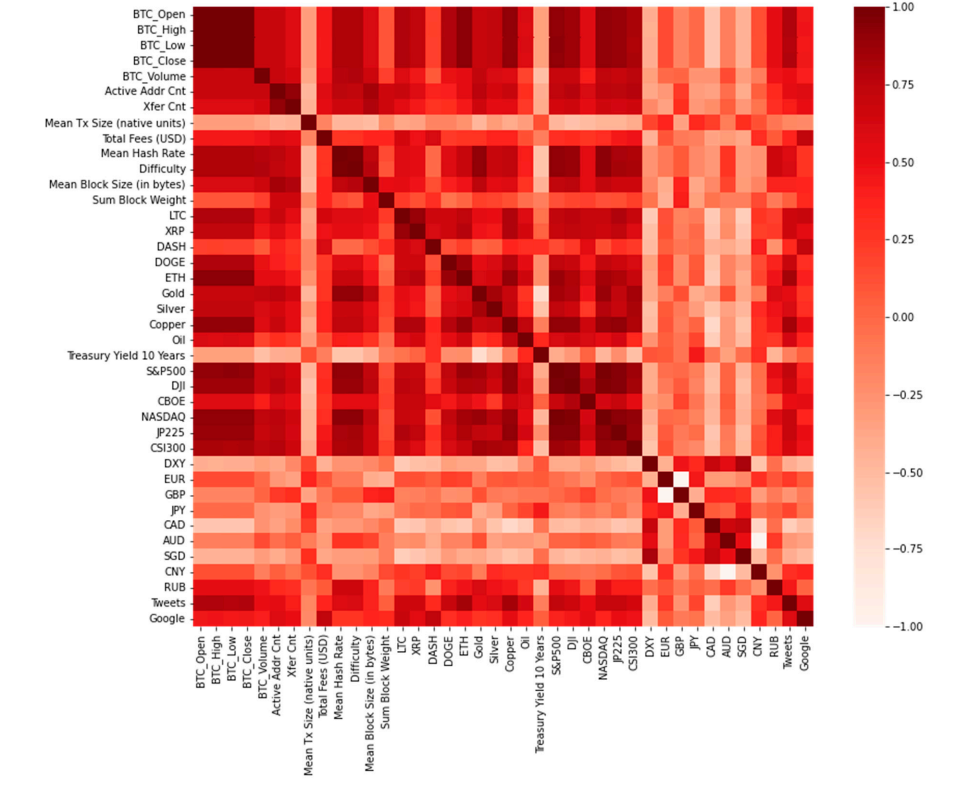
\includegraphics[width=\textwidth]{images/heatmap.png}
    \caption{Bản đồ nhiệt về mối tương quan giữa các biến}
    \label{fig:corr}
\end{figure}


Bản đồ nhiệt về mối tương quan (Hình \ref{fig:corr}) cho thấy Bitcoin có mối tương quan dương với nhiều loại tài sản khác, bao gồm các loại tiền mã hóa khác, giá hàng hóa, và các chỉ số thị trường chứng khoán. Điều này cho thấy rằng khi các thị trường này tăng trưởng, giá Bitcoin cũng có xu hướng tăng theo. Tuy nhiên, một điểm ngoại lệ quan trọng là mối tương quan nghịch giữa giá Bitcoin và lợi suất trái phiếu kho bạc Mỹ kỳ hạn 10 năm trong danh mục hàng hóa. Khi lợi suất trái phiếu tăng, giá Bitcoin có xu hướng giảm, điều này phản ánh dòng chảy vốn quay trở lại các tài sản an toàn hơn khi nền kinh tế có dấu hiệu cải thiện. Ngoài ra, mối tương quan âm giữa giá Bitcoin và tỷ giá hối đoái, đặc biệt là khi đồng USD mạnh lên, cũng là một xu hướng hợp lý, do giá trị của Bitcoin giảm khi đồng đô la trở nên hấp dẫn hơn. Điều đáng chú ý là tỷ giá đồng rúp Nga lại có mối tương quan dương cao với giá Bitcoin, có thể phản ánh tình trạng bất ổn kinh tế ở Nga dẫn đến việc dòng vốn dịch chuyển vào Bitcoin như một tài sản trú ẩn.

Một phát hiện thú vị khác là sự biến động của Bitcoin theo các ngày trong tuần. Biến động cực mạnh thường diễn ra vào thứ Tư, với phương sai lợi nhuận lớn nhất và những biến động hàng ngày lớn nhất, cả về tăng và giảm, đều xuất hiện vào ngày này. Ngược lại, vào cuối tuần, phương sai lợi nhuận giảm xuống và mức độ ổn định cao hơn so với các ngày trong tuần. Lợi nhuận trung bình hàng ngày của Bitcoin là 0,28\%, với biên độ tin cậy 95\% nằm trong khoảng [0,13\%, 0,43\%]. Đáng chú ý, lợi nhuận trung bình vào thứ Hai là cao nhất, trong khi vào Chủ Nhật là thấp nhất, cho thấy một xu hướng tăng giá mạnh vào đầu tuần. Xác suất tăng giá hàng ngày của Bitcoin là 54,57\%, với thứ Bảy và thứ Sáu là hai ngày có xác suất tăng cao nhất. Điều này cho thấy thị trường có những chu kỳ nhất định, có thể là do yếu tố giao dịch hoặc tác động từ các tin tức thị trường.

\begin{figure}[h]
    \centering
    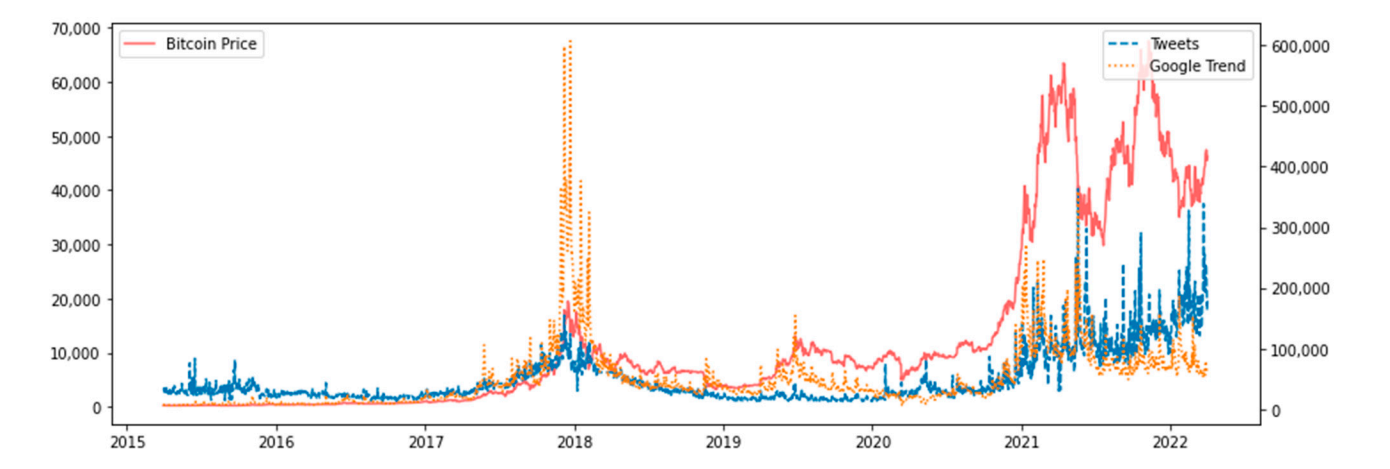
\includegraphics[width=\textwidth]{images/google_tweets_comparison.png}
    \caption{So sánh mức độ quan tâm của công chúng qua Google Trends và số lượng tweet hàng ngày với giá Bitcoin}
    \label{fig:interest_public}
\end{figure}

Liên quan đến mức độ quan tâm của công chúng, hai biến số quan trọng là xu hướng tìm kiếm trên Google và số lượng tweet hàng ngày (Hình \ref{fig:interest_public}) cũng có liên hệ chặt chẽ với biến động giá Bitcoin. Hai xu hướng chính có thể được rút ra: đầu tiên, đỉnh cao của Google Trends và số lượng tweet trùng khớp với những thời điểm Bitcoin đạt mức giá cao kỷ lục. Thứ hai, đỉnh cao nhất của Google Trends diễn ra vào cuối năm 2017, thời điểm Bitcoin đạt mốc giá quan trọng. Dù giá Bitcoin đã vượt ngưỡng 60.000 USD vào năm 2021, mức độ tìm kiếm trên Google vẫn không đạt đến đỉnh cao như năm 2017, cho thấy sự thay đổi trong mức độ quan tâm của công chúng đối với Bitcoin theo thời gian. Điều này có thể phản ánh sự bão hòa của thị trường tiền mã hóa hoặc sự thay đổi trong nhận thức của công chúng về Bitcoin.


% 
% \begin{savequote}[75mm] 
% Nulla facilisi. In vel sem. Morbi id urna in diam dignissim feugiat. Proin molestie tortor eu velit. Aliquam erat volutpat. Nullam ultrices, diam tempus vulputate egestas, eros pede varius leo.
% \qauthor{Quoteauthor Lastname} 
% \end{savequote}

% \chapter{Consectetuer adipiscing elit}

% \newthought{Lorem ipsum dolor sit amet}, consectetuer adipiscing elit. Morbi commodo, ipsum sed pharetra gravida, orci magna rhoncus neque, id pulvinar odio lorem non turpis. Nullam sit amet enim. Suspendisse id velit vitae ligula volutpat condimentum. Aliquam erat volutpat. Sed quis velit. Nulla facilisi. Nulla libero. Vivamus pharetra posuere sapien. Nam consectetuer. Sed aliquam, nunc eget euismod ullamcorper, lectus nunc ullamcorper orci, fermentum bibendum enim nibh eget ipsum. Donec porttitor ligula eu dolor. Maecenas vitae nulla consequat libero cursus venenatis. Nam magna enim, accumsan eu, blandit sed, blandit a, eros.

% \blindtext

% \section{This is section one}
% \blindtext
% \blindmathpaper

% \section{This is section two}
% \blindtext
% \blindmathpaper
\chapter{Kiến thức nền tảng}
\section{Mạng nơ-ron hồi quy}
\subsection{Dữ liệu tuần tự}
Dữ liệu tuần tự (Sequence data) là loại dữ liệu trong đó thứ tự của các điểm dữ liệu đóng vai trò quan trọng trong việc phân tích và dự đoán. Thông tin tại một thời điểm nhất định không tồn tại độc lập mà có sự phụ thuộc lẫn nhau giữa các thời điểm, thường là thông tin từ quá khứ ảnh hưởng đến tương lai. Dữ liệu tuần tự có thể gặp ở nhiều dạng bài toán khác nhau, từ chuỗi thời gian (time series), văn bản, chuỗi sự kiện, cho đến tín hiệu sinh học. Trong bài toán dự báo giá Bitcoin, dữ liệu tuần tự là dữ liệu giá của Bitcoin theo thời gian, nơi mà giá hiện tại có thể bị ảnh hưởng bởi các giá trước đó. Để xây dựng một mô hình dự báo chính xác, cần có khả năng học được mối quan hệ giữa các giá trong quá khứ và giá hiện tại. Đây là lý do tại sao Recurrent Neural Networks (RNN) trở nên phù hợp để xử lý bài toán này, vì RNN có khả năng ghi nhớ và học từ các dữ liệu tuần tự.
\subsection{Khái niệm}
Mạng nơ-ron hồi quy (Recurrent Neural Networks - RNN) là một loại mạng nơ-ron nhân tạo được thiết kế đặc biệt để xử lý dữ liệu tuần tự, như chuỗi thời gian, văn bản, hoặc tín hiệu âm thanh. Điểm đặc biệt của RNN là khả năng ghi nhớ thông tin từ quá khứ thông qua trạng thái ẩn (hidden state), điều này cho phép mô hình học các phụ thuộc dài hạn trong dữ liệu tuần tự. Tưởng tượng khi ta đang đọc một câu, mỗi từ ta đọc đều có mối liên hệ với các từ trước đó. RNN có khả năng duy trì thông tin này thông qua các bước thời gian, giúp nó trở nên hữu ích cho những bài toán liên quan đến dữ liệu tuần tự.
\subsection{Kiến trúc mạng nơ-ron hồi quy}
Mạng nơ-ron hồi quy (còn được gọi là RNN) là một lớp mạng neural đặc biệt, cho phép sử dụng đầu ra của một bước làm đầu vào cho bước tiếp theo, cùng với việc duy trì trạng thái ẩn qua các thời điểm. Điều này giúp RNN trở nên mạnh mẽ trong việc xử lý các dữ liệu tuần tự và có phụ thuộc lẫn nhau, như chuỗi thời gian hoặc văn bản.

\begin{figure}[h]
    \centering
    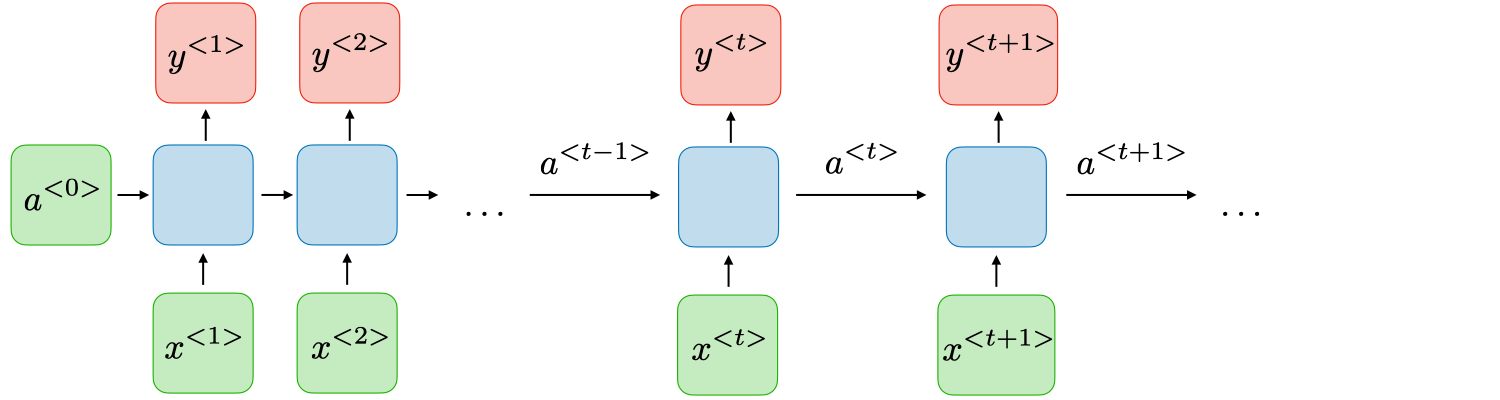
\includegraphics[width=1\textwidth]{images/LSTM/architecture-rnn-ltr.png}
    \caption{Cấu trúc của mạng RNN}
    \label{fig:rnn_architecture}
\end{figure}

Tại mỗi bước $t$, giá trị kích hoạt $a^{\langle t \rangle}$ và đầu ra $y^{\langle t \rangle}$ được biểu diễn như sau:

\begin{equation}
    a^{\langle t \rangle} = g_1 \Big( W_{aa} a^{\langle t-1 \rangle} + W_{ax} x^{\langle t \rangle} + b_a \Big)
\end{equation}

\begin{equation}
    y^{\langle t \rangle} = g_2 \Big( W_{ya} a^{\langle t \rangle} + b_y \Big)
\end{equation}

với $W_{ax}, W_{aa}, W_{ya}, b_a, b_y$ là các hệ số được chia sẻ tạm thời và $g_1, g_2$ là các hàm kích hoạt.

Giải nghĩa các biến
\begin{itemize}
    \item $x^{\langle t \rangle}$: Đầu vào tại thời điểm $t$, ví dụ như một phần của chuỗi dữ liệu.
    \item $a^{\langle t \rangle}$: Trạng thái ẩn tại thời điểm $t$, được tính dựa trên đầu vào hiện tại và trạng thái ẩn trước đó.
    \item $y^{\langle t \rangle}$: Đầu ra tại thời điểm $t$, có thể là giá trị dự đoán của mô hình.
    \item $W_{aa}$: Ma trận trọng số áp dụng cho trạng thái ẩn trước đó.
    \item $W_{ax}$: Ma trận trọng số áp dụng cho đầu vào tại thời điểm hiện tại.
    \item $W_{ya}$: Ma trận trọng số áp dụng cho trạng thái ẩn để tính đầu ra.
    \item $b_{a}$: Bias cho trạng thái ẩn.
    \item $b_{y}$: Bias cho đầu ra.
    \item $g_1, g_2$: Các hàm kích hoạt, ví dụ như hàm sigmoid, tanh hoặc ReLU, được sử dụng để tính toán các giá trị trạng thái ẩn và đầu ra.
\end{itemize}

\begin{figure}[h]
    \centering
    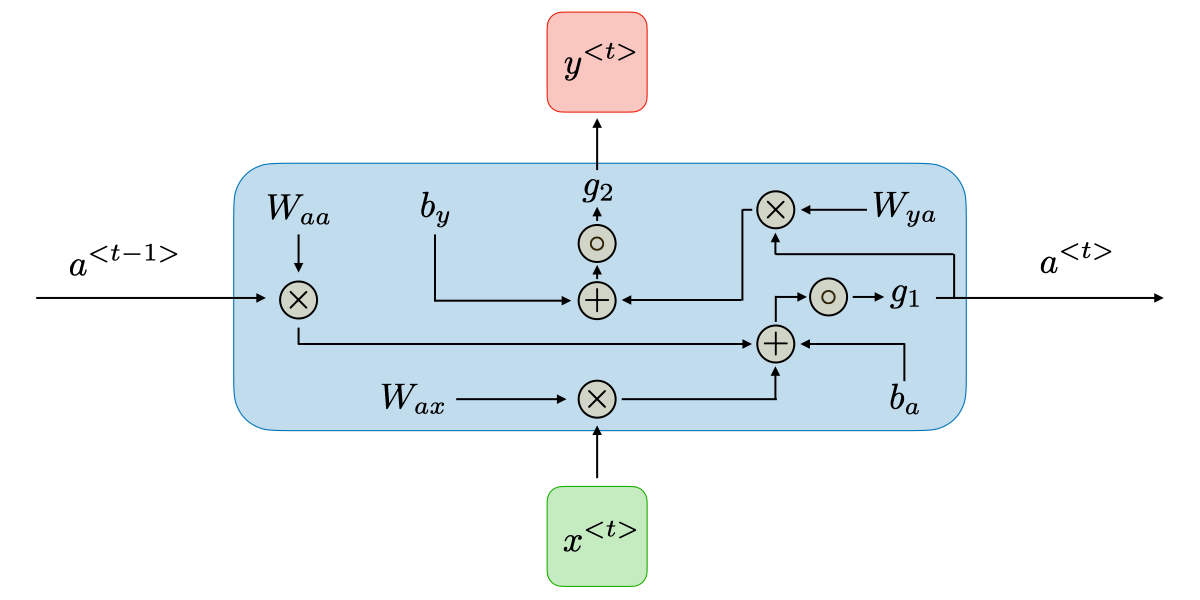
\includegraphics[width=1\textwidth]{images/LSTM/description-block-rnn-ltr.png}
    \caption{Chi tiết cấu trúc của RNN}
    \label{fig:rnn_hidden}
\end{figure}

Các hàm kích hoạt thường dùng trong các modules RNN được miêu tả như sau:

\begin{figure}[h!]
    \centering
    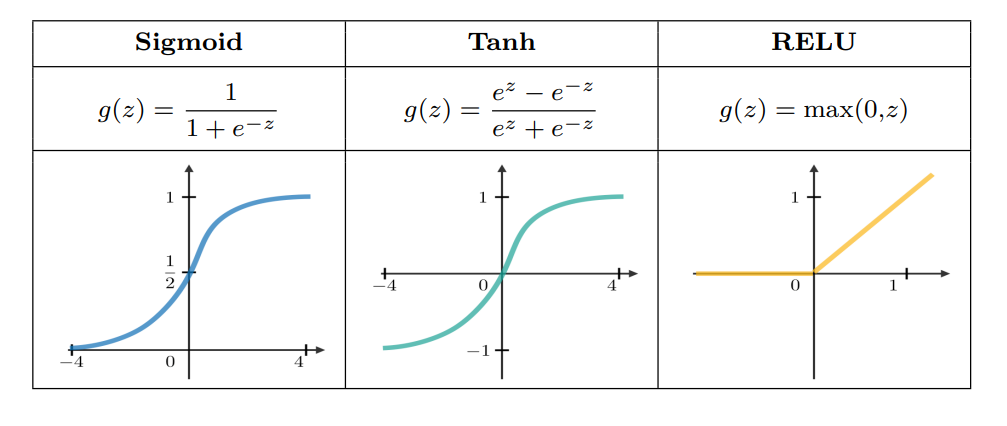
\includegraphics[width=\textwidth]{images/activation.png}
    \caption{Các hàm kích hoạt mà RNN hay sử dụng}
    \label{fig:activation_functions}
\end{figure}

\subsection{Ưu và nhược điểm của RNN}

\begin{table}[h]
    \centering
    \renewcommand{\arraystretch}{1} % tăng khoảng cách giữa các dòng
    \begin{tabular}{|p{7.5cm}|p{7.5cm}|}
        \hline
        \textbf{Ưu điểm} & \textbf{Hạn chế} \\ \hline
        \begin{itemize}
            \item Khả năng xử lí đầu vào với bất kì độ dài nào
            \item Kích cỡ mô hình không tăng theo kích cỡ đầu vào
            \item Quá trình tính toán sử dụng các thông tin cũ
            \item Trọng số được chia sẻ trong suốt thời gian
        \end{itemize} 
        & 
        \begin{itemize}
            \item Tính toán chậm
            \item Khó để truy cập các thông tin từ một khoảng thời gian dài trước đây
            \item Không thể xem xét bất kỳ đầu vào nào trong tương lai cho trạng thái hiện tại
        \end{itemize} \\ \hline
    \end{tabular}
    \caption{Ưu điểm và hạn chế của RNN}
    \label{tab:uudiem_hanche}
\end{table}

\subsection{Hàm mất mát}

Loss Function của RNN bằng tổng các Loss tại các Time-Step:
\begin{equation*}
    \mathcal{L}(\hat{y}, y) = \sum_{t=1}^{T_y} \mathcal{L}(\hat{y}^{\langle t \rangle}, y^{\langle t \rangle})
\end{equation*}

\subsection{Lan truyền ngược theo thời gian}

Lan truyền ngược theo thời gian (Backpropagation) được thực hiện tại mỗi Time-Step. Tại Time-Step $T$, đạo hàm của Loss Function $\mathcal{L}$ đối với ma trận trọng số $W$ được cho bởi công thức:
\begin{equation*}
    \frac{\partial \mathcal{L}^{(T)}}{\partial W} = \sum_{t=1}^{T} \frac{\partial \mathcal{L}^{(T)}}{\partial W}\Big|_{(t)}
\end{equation*}

\subsection{Xử lí phụ thuộc dài hạn}
Vanishing Gradient: Vanishing Gradient xảy ra khi giá trị của gradient trở nên cực kỳ nhỏ trong quá trình lan truyền ngược qua các lớp của mạng neural sâu. Khi gradient trở nên rất nhỏ, các trọng số của mạng không thể cập nhật hiệu quả, điều này khiến cho mạng không học được hoặc học rất chậm. Hiện tượng này đặc biệt phổ biến trong các mạng neural có nhiều lớp hoặc trong các mạng hồi quy (RNN) với chuỗi thời gian dài. Nguyên nhân chính của hiện tượng này là do các gradient bị nhân nhiều lần với các giá trị nhỏ hơn 1, dẫn đến giá trị gần bằng 0 khi chúng lan truyền ngược qua nhiều lớp.

Exploding Gradient: Exploding Gradient xảy ra khi giá trị của gradient trở nên quá lớn trong quá trình lan truyền ngược, dẫn đến sự cập nhật trọng số không ổn định hoặc thậm chí gây tràn số (overflow). Điều này làm cho mạng trở nên không ổn định và không thể hội tụ, thường xảy ra khi các gradient được nhân nhiều lần với các giá trị lớn hơn 1 qua nhiều lớp. Để khắc phục vấn đề này, một kỹ thuật thường được sử dụng là Gradient Clipping, nhằm giới hạn giá trị của gradient trong một phạm vi nhất định, giúp đảm bảo quá trình học của mạng được ổn định hơn.

Giống như nhiều mô hình học sâu khác, hiện tượng Vanishing và Exploding Gradient cũng xuất hiện trong RNN, gây khó khăn cho việc ghi nhớ các trạng thái từ những bước thời gian xa. Nguyên nhân chính của vấn đề này là do việc nhân gradient theo hàm mũ, dẫn đến sự tăng hoặc giảm đột ngột khi số lượng lớp mạng tăng lên, khiến quá trình học trở nên không ổn định.

Sử dụng ReLU chúng ta đã giải quyết được khá tốt vấn đề Vanishing Gradient. Còn đối với Exploring Gradient, chúng ta có thể sử dụng Gradient Clipping.

\begin{figure}[h!]
    \centering
    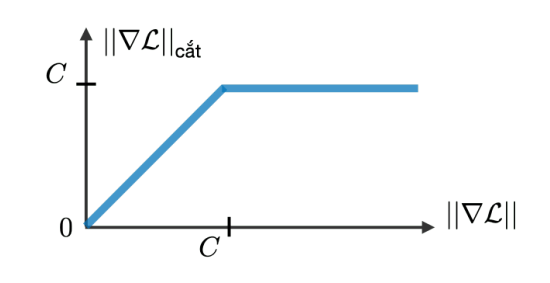
\includegraphics[width=0.8\textwidth]{images/gradient.png}
    \caption{Gradient Clipping để giới hạn Gradient}
    \label{fig:gradient_clipping}
\end{figure}

Gradient clipping là một kĩ thuật được sử dụng để giải quyết vấn đề exploding gradient xảy ra khi thực hiện lan truyền ngược. Bằng việc giới hạn giá trị lớn nhất cho gradient, hiện tượng này sẽ được kiểm soát trong thực tế.

\section{Bộ nhớ dài-ngắn hạn (LSTM)}
Bộ nhớ dài-ngắn hạn (Long Short Term Memory) là một phiên bản cải tiến của RNN, giúp mô hình dễ dàng ghi nhớ dữ liệu quá khứ hiệu quả hơn. Với LSTM, vấn đề Vanishing Gradient trong RNN được giải quyết tốt hơn, nhờ đó mô hình có khả năng lưu giữ và học từ thông tin ở các bước thời gian xa. LSTM đặc biệt phù hợp cho các bài toán phân loại, xử lý, và dự đoán chuỗi thời gian có độ dài không cố định. Mô hình này cũng được huấn luyện thông qua quá trình Backpropagation.

Kiến trúc của mạng LSTM bao gồm nhiều lớp (Layers), mỗi lớp được cấu thành từ các đơn vị nhỏ gọi là Cell. Mỗi Cell được mô tả bởi hai bộ nhớ quan trọng: Cell State (\(C\)) và Hidden State (\(h\)).

- \textbf{Hidden State - h,H}: Bộ nhớ ngắn hạn (\textit{working memory}), lưu giữ thông tin từ Cell ngay trước Cell hiện tại. Hidden State tồn tại trong cả RNN và LSTM, và cũng chính là Output của mỗi Cell trong RNN/LSTM.

- \textbf{Cell State - C}: Bộ nhớ dài hạn (\textit{long-term memory, memory cell}), có nhiệm vụ lưu trữ thông tin từ nhiều Cells trong quá khứ. Bộ nhớ này chỉ tồn tại trong LSTM, giúp mạng duy trì thông tin cần thiết qua các bước thời gian.

Xét một Cell tại thời điểm hiện tại (\(C_t, h_t\)) trong LSTM, luồng dữ liệu đi qua Cell này sẽ lần lượt trải qua ba cổng chính như sau:

- \textbf{Forget gate}: Cổng này quyết định thông tin nào từ Cell trước đó (\(C_{t-1}\)) cần được giữ lại hay loại bỏ. Thông tin từ Hidden State trước (\(h_{t-1}\)) và từ Input hiện tại (\(x_t\)) được đưa qua hàm Sigmoid, tạo ra một giá trị từ 0 đến 1. Giá trị càng gần 0 cho thấy thông tin ít quan trọng và có thể bỏ qua, trong khi giá trị càng gần 1 cho thấy thông tin quan trọng cần được giữ lại.

\begin{figure}[h!]
    \centering
    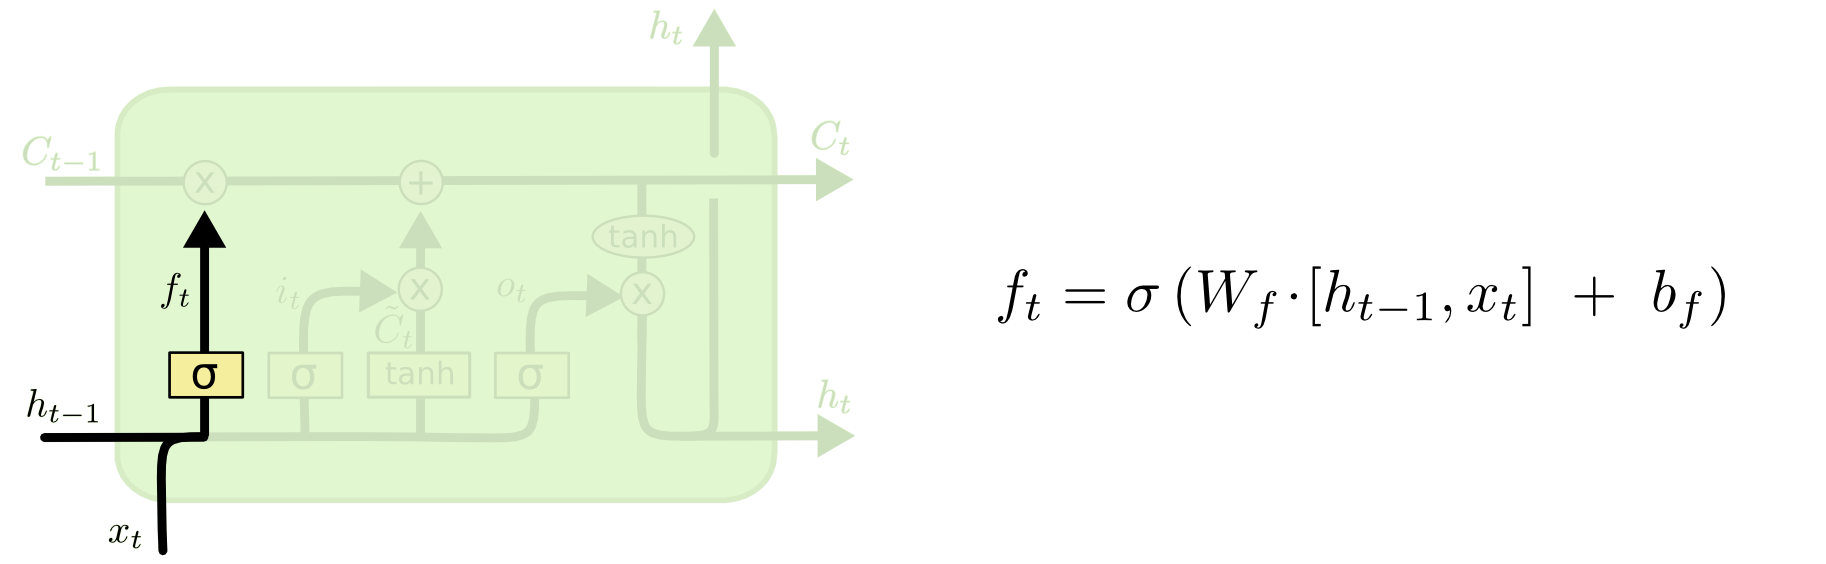
\includegraphics[width=\textwidth]{images/LSTM/lstm-forget-f.png}
    \caption{Minh họa Forget Gate trong LSTM}
    \label{fig:lstm_cell}
\end{figure}

\begin{equation*}
    f_t = \sigma \left( W_f \cdot [h_{t-1}, x_t] + b_f \right) = \sigma (W_{xf} X_t + W_h h_{t-1} + b_f)
\end{equation*}

- \textbf{Input gate}: Cổng này quyết định giá trị nào từ Hidden State trước (\(h_{t-1}\)) và thông tin từ Input hiện tại (\(x_t\)) sẽ được đưa vào Cell hiện tại. Để thực hiện điều này, cổng sử dụng kết hợp hai hàm Sigmoid và Tanh. Tương tự như Forget Gate, thông tin từ Hidden State trước (\(h_{t-1}\)) và từ Input hiện tại (\(x_t\)) được đưa qua hàm Sigmoid, tạo ra một giá trị từ 0 đến 1, phản ánh mức độ quan trọng của thông tin—càng gần 0 thì thông tin càng ít quan trọng, càng gần 1 thì thông tin càng quan trọng. Tiếp theo, hàm Tanh tạo ra một vector ứng cử cho Cell State hiện tại (\(\tilde{C_t}\)). Output từ hai hàm này được nhân với nhau để tính toán Cell State của thời điểm hiện tại.


\begin{figure}[h!]
    \centering
    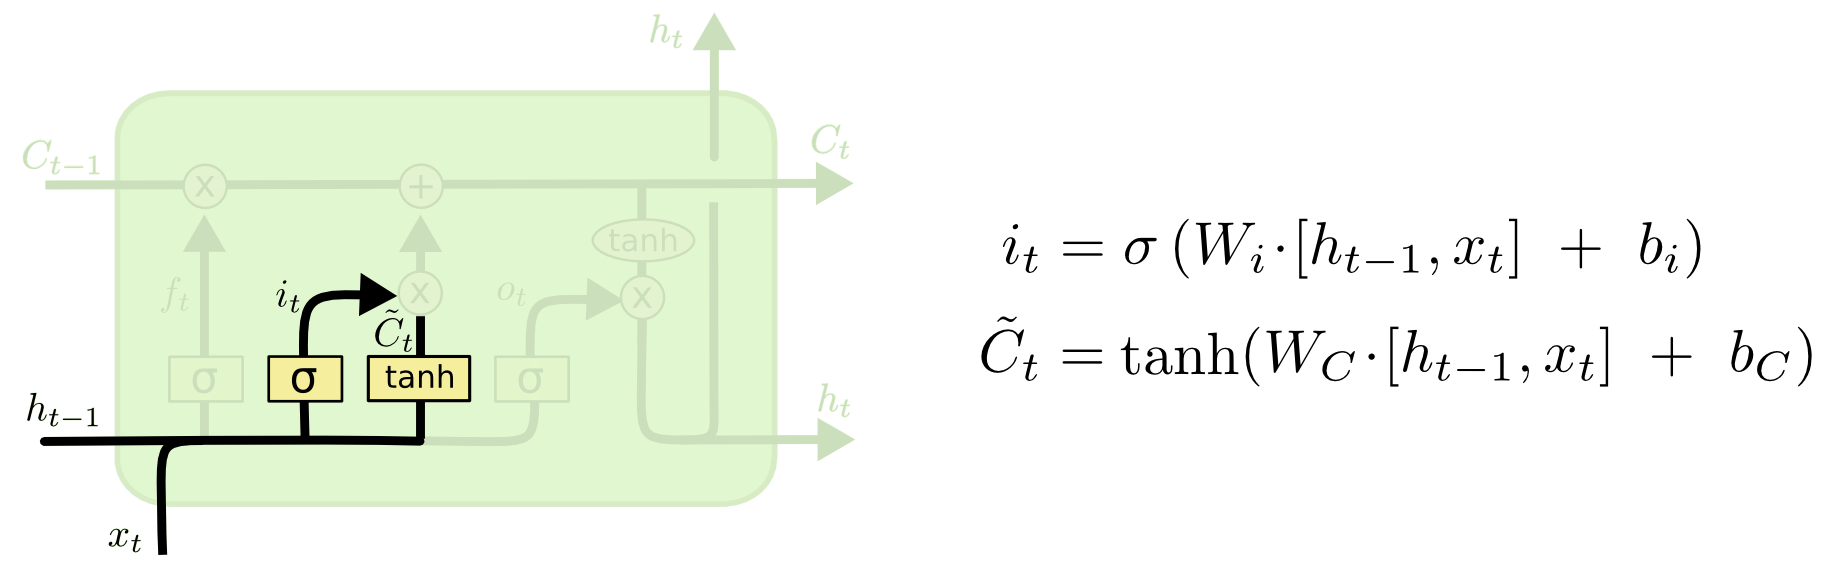
\includegraphics[width=\textwidth]{images/LSTM/lstm-input-i.png}
    \caption{Minh họa Input Gate trong LSTM}
    \label{fig:lstm_input_gate}
\end{figure}

\begin{equation*}
    i_t = \sigma \left( W_i \cdot [h_{t-1}, x_t] + b_i \right) = \sigma (W_{xi} X_t + W_h h_{t-1} + b_i)
\end{equation*}

\begin{equation*}
    \tilde{C_t} = \tanh \left( W_c \cdot [h_{t-1}, x_t] + b_c \right) = \tanh (X_t W_{xc} + h_{t-1} W_{hc} + b_c)
\end{equation*}

Đến đây, ta đã có thể tính được Cell State hiện tại:

\begin{figure}[h!]
    \centering
    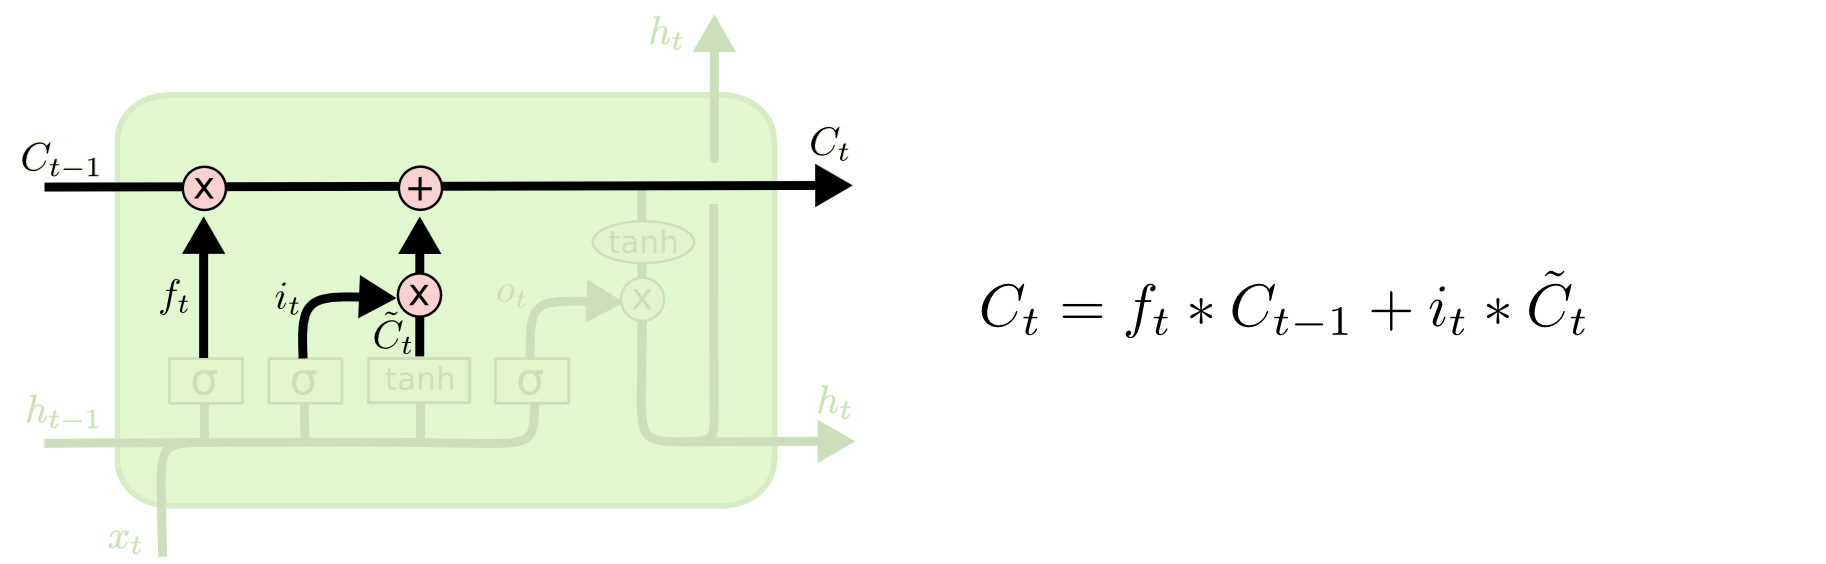
\includegraphics[width=\textwidth]{images/LSTM/lstm-cellstate-c.png}
    \caption{Minh họa tính toán Cell State hiện tại}
    \label{fig:lstm_cell_state}
\end{figure}

\begin{equation*}
    C_t = f_t * C_{t-1} + i_t * \tilde{C_t}
\end{equation*}

Chú giải về các phép toán:

\begin{itemize}
    \item \(\otimes\): Element-wise multiplication
    \item \(\oplus\): Element-wise addition
\end{itemize}

Chúng ta nhân trạng thái của Cell trước đó với \(f_t\) rồi cộng với \(i_t * \tilde{C_t}\):

\begin{equation*}
    C_t = f_t * C_{t-1} + i_t * \tilde{C_t}
\end{equation*}

- \textbf{Output gate}: Cổng này xác định thông tin nào sẽ được truyền ra làm đầu ra (\(h_t\)). Tương tự như hai cổng trước đó, thông tin từ Hidden State trước (\(h_{t-1}\)) và từ Input hiện tại (\(x_t\)) được đi qua hàm Sigmoid, tạo ra một giá trị từ 0 đến 1. Giá trị này càng gần 0 thì thông tin càng kém quan trọng, ngược lại, giá trị càng gần 1 cho thấy thông tin càng quan trọng. Sau đó, Cell State được chuyển qua hàm Tanh để đưa giá trị về khoảng \([-1, 1]\).

\begin{figure}[h!]
    \centering
    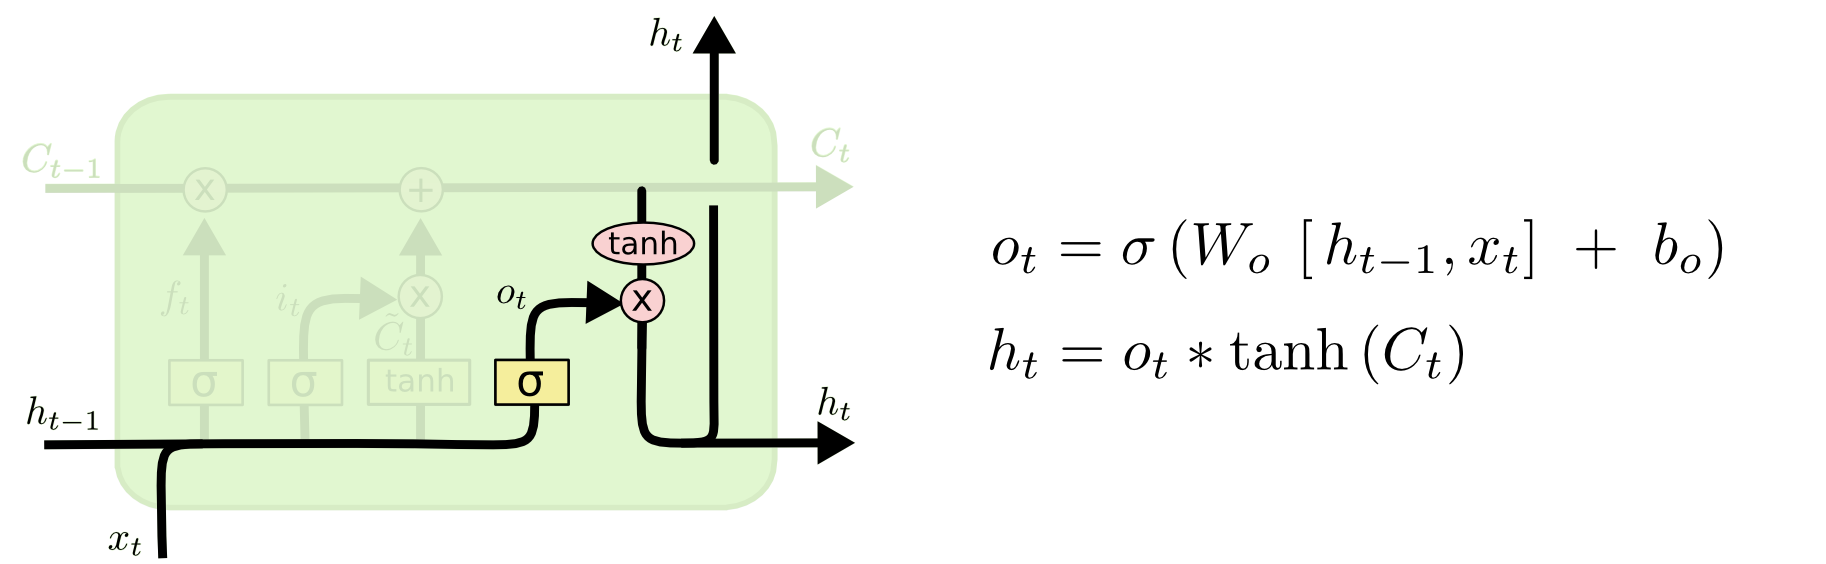
\includegraphics[width=\textwidth]{images/LSTM/lstm-output-o.png}
    \caption{Minh họa Output Gate trong LSTM}
    \label{fig:lstm_output_gate}
\end{figure}

Output của Cell được tính như sau:

\begin{equation*}
    o_t = \sigma \left( W_o \cdot [h_{t-1}, x_t] + b_o \right) = \sigma (W_{xo} X_t + W_h h_{t-1} + b_o)
\end{equation*}

\begin{equation*}
    h_t = o_t * \tanh (C_t)
\end{equation*}

\section{Gated Recurrent Unit (GRU)}
Gated Recurrent Unit (GRU) là một phiên bản cải tiến khác của RNN, được phát triển nhằm giải quyết vấn đề Vanishing Gradient và tăng hiệu suất học của mạng. GRU có cấu trúc đơn giản hơn LSTM khi chỉ sử dụng hai cổng: Reset Gate và Update Gate. Nhờ thiết kế tinh gọn này, GRU thường yêu cầu ít tài nguyên tính toán hơn nhưng vẫn đạt được hiệu quả tương đương với LSTM trong nhiều trường hợp. Điều này giúp GRU trở thành lựa chọn phù hợp cho các bài toán yêu cầu khả năng xử lý nhanh hoặc trên các thiết bị có hạn chế về tài nguyên.

\begin{figure}[h!]
    \centering
    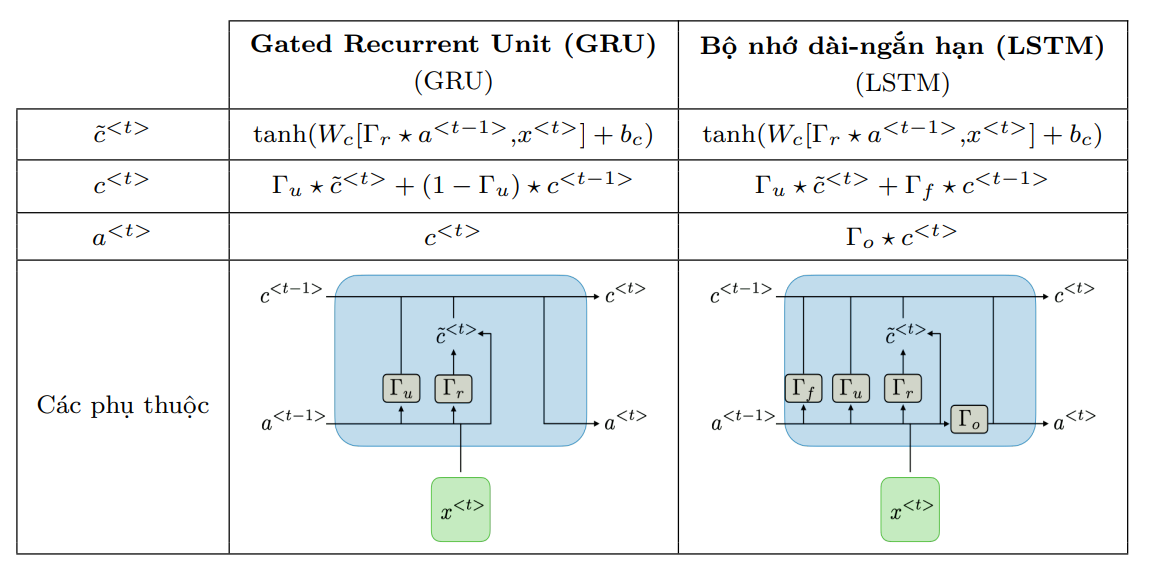
\includegraphics[width=0.7\textwidth]{images/LSTM/lstm_summary.png}
    \caption{Tổng kết các phương trình đặc trưng của LSTM và GRU}
    \label{fig:lstm_summary}
\end{figure}







% Phần cây quyết định và rừng ngẫu nhiên (chưa thêm ảnh và chưa link phương trình, chưa có reference)
\section{Cây quyết định}

\subsection{Giới thiệu}
Cây quyết định là một mô hình có cấp bậc (hierarchichal) có giám sát (supervised), trong đó những vùng cục bộ được xác định bằng việc chia ra một cách hồi quy.
Cây quyết định gồm có 2 thành phần chính: nút quyết định (decision nodes) và các lá kết thúc (terminal leaves).
Mỗi nút quyết định $m$ chứa một hàm thử $f_m(\mathbf{x})$ với kết quả rời rạc được đánh nhãn cho các nhánh.
\begin{figure}[hbpt]
    \centering
    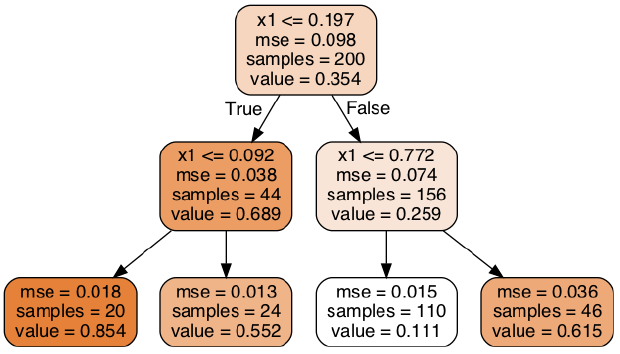
\includegraphics[width=\linewidth]{figures/decision_tree.png}
    \caption{Ví dụ về một cây quyết định}
    \label{fig:decision_tree_example}
\end{figure}

\subsection{Cây đơn biến}
Mỗi nút trong cây đơn biến \textbf{chỉ sử dụng một biến (feature / attribute) trong chiều dữ liệu đầu vào.} Đây cũng là cài đặt mặc định của \textit{scikit-learn} \cite{aurelien2019handsonml}.
\begin{itemize}
    \item Nếu biến được sử dụng, ký hiệu $x_j$ là rời rạc thì nút sẽ sử dụng một trong số $n$ giá trị rời rạc đó và nhánh đó sẽ có khả năng được chia ra thành $n$ nhánh con (gọi là $n$-way split).
    \item Nếu biến được sử dụng là biến số thì nó nên được rời rạc hóa, nhưng nếu là số có thứ tự (liên tục) thì phép thử được sử dụng sẽ là phép so sánh, và vì vậy nó là 2-way split.
\end{itemize}

\begin{equation} f_m(\mathbf{x}): x_j - w_{m0} > 0 \end{equation}

\subsection{Cây phân loại}
Với cây phân loại thì chất lượng của mỗi lần chia nhánh sẽ được đo bằng \textit{độ hỗn loạn}. Độ hỗn loạn càng thấp thì tức là lần chia nhánh càng tốt.
Trong một nút $m$, ta ký hiệu $N_m$ là số lượng phần tử trong tập huấn luyện đã cập đến nút $m$ (Với nút gốc thì $N_{root} = N$), $N^i_m$ trong số $N_m$ thuộc về lớp $C_i$. Một phần tử trong tập huấn luyện cập đến nút $m$ thì xác suất để nó thuộc lớp $C_i$ là

\begin{equation} \hat{P}(C_i|\mathbf{x}, m) \equiv p^i_m = \frac{N^i_m}{N_m} \end{equation}

Nút $m$ thuần khi $p^i_m$ với tất cả mọi $i$ là 0 hoặc 1 (tức là xác suất để vào các lớp là 0 hoặc 1). 0 khi không có phần tử thuộc lớp $C_i$ nào cập đến nút $m$, và 1 khi tất cả đều cập đến nút $C_i$. Nếu nút ổn định thì ta không cần chia thêm nút con (nhánh con) cho nó nữa. Một cách để đo độ hỗn loạn là \textit{entropy} - được tính theo công thức sau:

\begin{equation} I_m = -\sum_{i = 1}^{K} {p^i_m \log_2(p^i_m)} \end{equation}

\begin{figure}
    \centering
    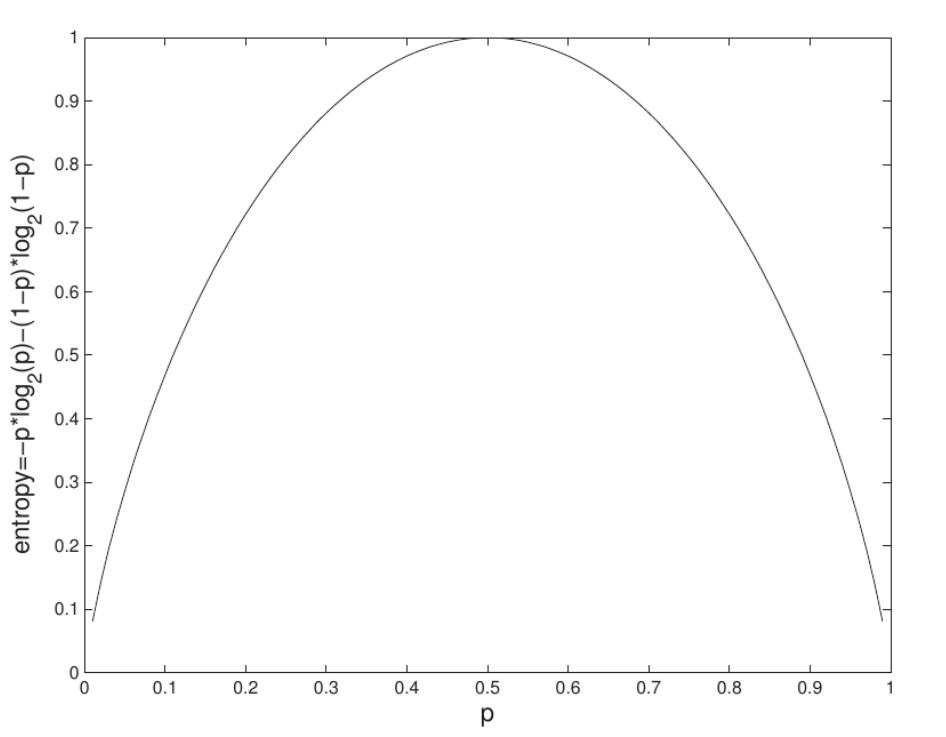
\includegraphics[width=\linewidth]{figures/entropy_graph.png}
    \caption{Đồ thị của hàm entropy}
    \label{fig:entropy_graph}
\end{figure}


Một đô đo sự hỗn loạn khác cũng được sử dụng phổ biến là chỉ số Gini:

\begin{equation} \phi(p, 1 - p) = 2p(1-p) \end{equation}

Nếu nút $m$ không thuần, thì mẫu dữ liệu cần được chia nhỏ để giảm độ hỗn loạn, và ta sẽ có phương án chia tùy thuộc vào dữ liệu. Trong các phương án được xét, ta cần tìm cách để giảm thiểu được độ hỗn loạn, để cho các nhánh sau ta không cần chia thêm nhiều lần nữa. Tất nhiên đây chỉ là \textbf{tối ưu cục bộ}, và ta không thể đảm bảo tìm ra được cây nhỏ nhất.
Ví dụ, ở nút $m$, $N_{mj}$ trong số $N_m$ phần tử theo nhánh $j$, đây là các phần tử $\mathbf{x}^t$ mà kết quả của phép thử $f_m(\mathbf{x}^t)$ trả về kết quả $j$. \textit{Đối với thuộc tính rời rạc với $n$ lớp, ta sẽ có $n$ kết quả; với một thuộc tính số, ta sẽ có 2 kết quả và giả sử có $n$ phần tử thì sẽ có $n - 1$ khe để ta có thể chia chúng thành hai tập}; cả hai trường hợp đều thỏa mãn $\sum_{j=1}^{n} N_{mj} = N_m$. $N^i_{mj}$ trong số $N_{mj}$ phần tử thuộc về lớp $C_i$: $\sum_{i=1}^{K} N^{i}_{mj} = N_{mj}$. Tương tự, $\sum_{j=1}^{n} N^i_{mj} = N^i_m$.

Cho nút $m$, kết quả của phép thử là $j$, vậy xác suất một phần tử được xác định vào lớp $C_i$ là:

\begin{equation} \hat{P}(C_i|\mathbf{x}, m, j) \equiv p^i_{m, j} = \frac{N^i_{m, j}}{N_{m, j}} \end{equation}

và độ hỗn tạp sau khi chia nhánh là:

\begin{equation} I'_m = -\sum^n_{j=1}\frac{N_{mj}}{N_m} \sum_{i = 1}^{K} {p^i_{mj} \log_2(p^i_{mj})} \end{equation}

Dưới đây là mã giả dạng Python để ta có thể hình dung ra được cách xây dựng một cây quyết định từ tập đầu vào \cite{alpaydin2010introml}:

\begin{algorithm}[H]
    \caption{Decision Tree Generation}
    \SetKwFunction{GenerateTree}{GenerateTree}
    \SetKwFunction{SplitAttribute}{SplitAttribute}
    \SetKwFunction{SplitEntropy}{SplitEntropy}
    \SetKwFunction{NodeEntropy}{NodeEntropy}
    \SetKwProg{Fn}{Function}{:}{}
    
    \Fn{\GenerateTree{$X$}}{
        \eIf{\NodeEntropy{X} $< \theta_i$}{
            Create leaf labeled by majority class in $X$\;
            \Return\;
        }{
            $i \gets$ \SplitAttribute{$X$}\;
            \For{each branch of $x_i$}{
                Find $X_i$ falling in branch\;
                \GenerateTree{$X_i$}\;
            }
        }
    }
    
    \Fn{\SplitAttribute{$X$}}{
        $minEntropy \gets \infty$\;
        \For{all attributes $i = 1$ to $d$}{
            \If{$x_i$ is discrete with $n$ values}{
                Split $X$ into $X_1, \ldots, X_n$ by $x_i$\;
                $e \gets$ \SplitEntropy{$X_1, \ldots, X_n$}\;
                \If{$e < minEntropy$}{
                    $minEntropy \gets e$\;
                    $bestF \gets i$\;
                }
            }
            \If{$x_i$ is numeric}{
                \For{all possible splits}{
                    Split $X$ into $X_1, X_2$ on $x_i$\;
                    $e \gets$ \SplitEntropy{$X_1, X_2$}\;
                    \If{$e < minEntropy$}{
                        $minEntropy \gets e$\;
                        $bestF \gets i$\;
                    }
                }
            }
        }
        \Return $bestF$\;
    }
\end{algorithm}

Vậy là với mỗi thuộc tính, rời rạc hay liên tục, phân mục hay số, thì ta sẽ tìm ra cách phân chia làm cho entropy trở nên nhỏ nhất. Đây là cơ sở của thuật toán cây phân loại và hồi quy (Classification And Regression Tree - CART).

\subsection{Cây hồi quy}
Cây hồi quy được xây dựng tương tự như cây phân loại, thay vì sử dụng độ hỗn loạn thì ta sẽ sử dụng một độ đo khác làm thang đo cho việc phân nhánh.
Giả sử trong nút $m$, $X_m$ là tập con của $X$ cập đến nút $m$ (tức là các phần tử được phân vào nút $m$ khi duyệt qua cây).

\begin{equation} b_m(x) = \begin{cases} 1 & \text{if } x \in X_m: \, x \text{ cập đến nút  } m\\ 0 & \text{ngược lại} \end{cases} \end{equation}

Trong cây hồi quy, chất lượng của một lần chia nhánh sẽ được đo bằng trung bình sai số bình phương (Mean Squared Error). Nếu ta ký hiệu $g_m$ là giá trị được ước lượng cho nút m thì

\begin{equation} E_m = \frac{1}{N_m} \sum_t{(r^t - g_m)^2 \cdot b_m(\mathbf{x}^t)} \end{equation}

Với $N_m = |{X_m}| = \sum_t{b_m(\mathbf{x}^t)}$.
Phương trình (6) sẽ thể hiện phương sai của kết quả thực với đầu ra trong nút $m$.
Trong một nút, ta dùng trung bình của các kết quả đầu ra (trung vị nếu có quá nhiều nhiễu)

\begin{equation} g_m = \frac{\sum_t {b_m (x_t)r^t}}{\sum_t {b_m (x_t)}} \end{equation}

Nếu tại một nút, sai số là chấp nhận được (tức là $E_m < \theta_r$ nào đó) thì một nút lá sẽ được tạo ra và lưu $g_m$ lại nút lá đó.
Nếu sai số không đạt yêu cầu, thì dữ liệu cập đến nút m sẽ tiếp tục được phân chia sao cho tổng sai số cho từng nhánh là thấp nhất. Giống với cây phân loại, ta sẽ đi tìm cách chia một thuộc tính nào đó sao cho sai số trung bình là nhỏ nhất, và tiếp tục công việc đó với các nhánh con.
Giả sử $X_{mj}$ là tập con của $X_m$ theo nhánh $j$. $\bigcup_{j=1}^{n} X_{mj} = X_{m}$ (tức là hội của phần tử theo mỗi nhánh $j$ từ $1$ đến $n$ sẽ là tập hợp các phần tử (tập mẹ) đạt đến nhánh $m$).
Ta định nghĩa

\begin{equation} b_{mj}(x) = \begin{cases} 1 & \text{if } x \in X_{mj}: \, x \text{ cập đến nút  } m \text {  và theo nhánh j}\\ 0  & \text{ngược lại} \end{cases} \end{equation}

$g_{mj}$ là giá trị được ước lượng cho nhánh $j$ của nút $m$.

\begin{equation} g_{mj} = \frac{\sum_t {b_{mj} (x_t)r^t}}{\sum_t {b_{mj} (x_t)}} \end{equation}

Và sai số sau khi chia nhánh là

\begin{equation} E'_m = \frac{1}{N_m}\sum_j \sum_t{(r^t - g_{mj})^2 \cdot b_{mj}(\mathbf{x}^t)} \end{equation}

Độ suy giảm sai số của một nhánh được chỉ ra ở phương trình (6) và (10). Ta sẽ đi tìm cách phân nhánh nào mà sai số ở phương trình (10) là nhỏ nhất. Trong đoạn mã giả mô phỏng, \texttt{node\_entropy(X)} và \texttt{split\_entropy([X])} sẽ được thay bằng việc tính toán sai số bình phương trung bình.

Vấn đề khi đặt ra ngưỡng sai số hoặc ngưỡng ổn định của dữ liệu $\theta_i$, ta phải chọn một mức phù hợp vì khi $\theta_i$ nhỏ thì sai số sẽ phải nhỏ và mô hình sẽ xảy ra tình trạng quá khớp (overfitting) và nếu đặt ở ngưỡng quá cao thì mô hình sẽ trở nên không hiệu quả (underfitting).

Một cách để giải quyết vấn đề là ta cắt tỉa các nút (tức là hủy phân nhánh nữa) - được đề cập ở phần tiếp theo.
\begin{figure}
    \centering
    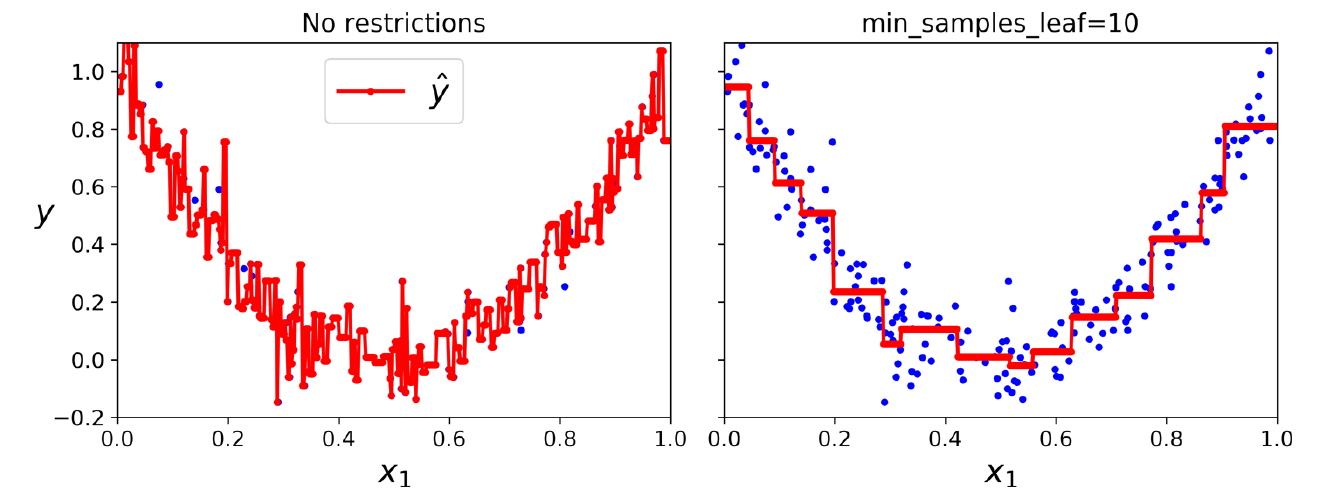
\includegraphics[width=\linewidth]{figures/dt_overfit1.png}
    \caption{Hình minh họa về việc overfitting ở cây quyết định khi độ sâu không bị giới hạn}
    \label{fig:dt_overfit1}
\end{figure}
\begin{figure}
    \centering
    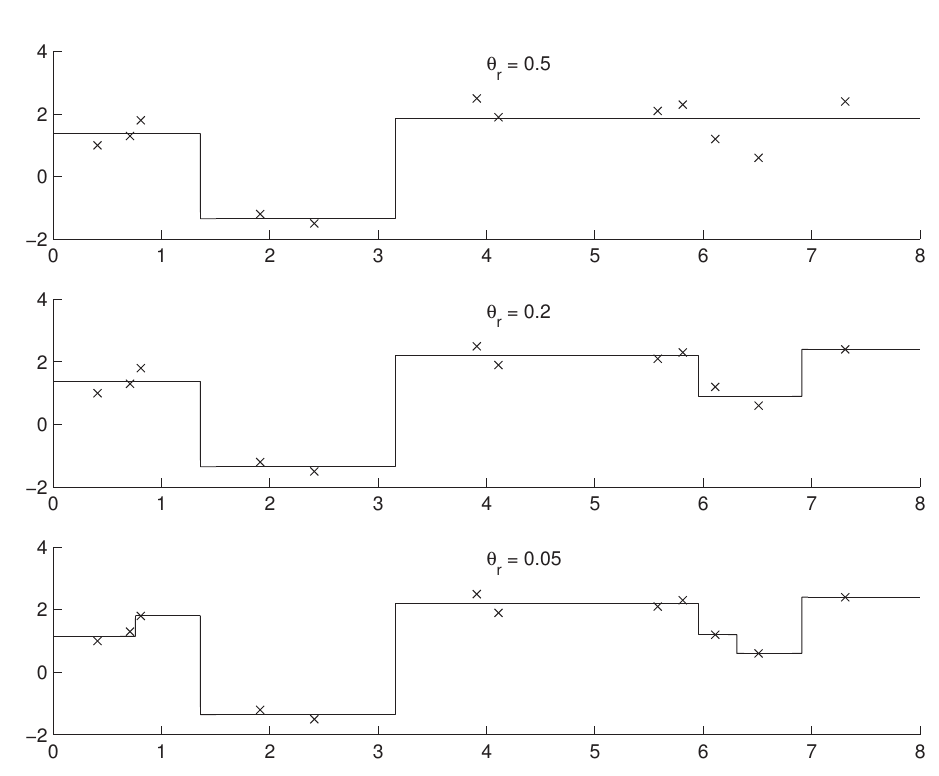
\includegraphics[width=0.7\linewidth]{figures/dt_overfit2.png}
    \caption{Hình minh họa fitting ở cây quyết định khi $\theta$ được đặt với nhiều giá trị khác nhau}
    \label{fig:dt_overfit2}
\end{figure}
\subsection{Cắt tỉa - Pruning}
Thường thì một nút sẽ không được chia nhỏ thêm nếu số lượng mẫu huấn luyện đến nút đó nhỏ hơn một tỷ lệ nhất định của tập huấn luyện - ví dụ, 5 phần trăm - bất kể độ không thuần hay sai số. Ý tưởng ở đây là bất kỳ quyết định nào dựa trên quá ít mẫu sẽ gây ra sự biến động và do đó làm tăng lỗi tổng quát hóa. Việc dừng quá trình xây dựng cây sớm trước khi cây được hoàn thiện được gọi là \textbf{cắt tỉa sớm (prepruning)}.
Một phương pháp để có được cây đơn giản hơn là \textbf{cắt tỉa sau (postpruning)}, điều này trên thực tế \textit{hoạt động hiệu quả hơn} so với cắt tỉa sớm (prepruning). Chúng ta đã thấy trước đó rằng quá trình xây dựng cây là tham lam, và ở mỗi bước, chúng ta đưa ra một quyết định, cụ thể là tạo ra một nút quyết định và tiếp tục mà không quay lại để thử các lựa chọn thay thế. Ngoại lệ duy nhất là \textbf{cắt tỉa sau (postpruning)}, trong đó chúng ta cố gắng tìm và cắt tỉa những nhánh con không cần thiết.

Với cắt tỉa sau, ta sẽ cho phép cây phát triển đầy đủ, đến khi tất cả các lá kết thúc đều thuần và không xuất hiện lỗi huấn luyện. Sau đó, ta sẽ tìm các cây con gây ra hiện tượng quá khớp và cắt tỉa chúng. Từ tập huấn luyện ban đầu, ta sẽ tạo thêm một \textbf{tập cắt tỉa} (pruning set) không dùng cho huấn luyện. Với mỗi cây con (nút con bên trong cây quyết định), thay thế nó bằng một lá nhãn. \textit{Lá này được gắn nhãn với lớp phổ biến nhất (trung bình với bài toán hồi quy) của các mẫu dữ liệu được phân loại vào cây con đó}. Nếu lá nhãn không hoạt động kém hơn cây con trên tập cắt tỉa, chúng ta cắt tỉa cây con và giữ lá nhãn; nếu không, chúng ta giữ cây con.

\subsection{Cây đa biến}
\textbf{Cây quyết định đơn biến} chỉ sử dụng một chiều đầu vào tại mỗi điểm phân chia. Trong \textbf{cây quyết định đa biến}, tại một nút quyết định, tất cả các chiều đầu vào có thể được sử dụng, do đó nó tổng quát hơn. Khi tất cả các đầu vào đều ở dưới dạng số, một \textbf{nút đa biến tuyến tính nhị phân} được định nghĩa là

\begin{equation} f_m(\mathbf{x}): \mathbf{w}_m^t\mathbf{x} + w_{m0} > 0 \end{equation}

Vì nút đa biến tuyến tính lấy tổng trọng số nên các thuộc tính rời rạc nên được mã hóa thành 0/1.
Tuy nhiên, một khó khăn mà ta gặp phải nữa, đó là ở một nút quyết định thì ta sẽ có rất nhiều cách chọn thuộc tính và giá trị thuộc tính để có thể chia nhánh. Ví dụ nếu tập dữ liệu có $d$ thuộc tính, và ta có $N_m$ phần tử cập đến nút m, thì khi quyết định chia ta sẽ có $2^d$ cách chọn thuộc tính, và với mỗi cách chọn thuộc tính ta lại có $\binom{N_m}{d}$ cách chia tập dữ liệu thành các khoảng. Vì vậy tìm kiếm thủ công là không khả thi. Một trong các giải pháp đã được đề cập là thuật toán OC1 \cite{Murthy1993oc1}.

\section{Rừng ngẫu nhiên - Random Forest}
Đây là một phương pháp học kết hợp các cây quyết định, và hầu hết được huấn luyện theo phương pháp tổng hợp khởi động có lặp (bootstrap aggregating - bagging) hoặc tổng hợp không thay thế (pasting). Vậy bagging và pasting có nghĩa là gì?
Trong \textbf{Bagging}, các tập dữ liệu con được chọn ngẫu nhiên từ tập dữ liệu gốc \textbf{có phép thay thế} (tức là một mẫu có thể xuất hiện nhiều lần trong các tập con). Sau đó, một mô hình riêng biệt được huấn luyện trên từng tập dữ liệu con, và kết quả cuối cùng được tổng hợp lại (\textit{trung bình đối với các bài toán hồi quy hoặc bỏ phiếu đa số đối với các bài toán phân loại}).
Lợi ích của Bagging là giảm phương sai của mô hình và cải thiện độ chính xác bằng cách tận dụng nhiều mô hình độc lập. Với Bagging, thống kê chỉ ra rằng, vì có những phần tử dữ liệu được chọn lại nên sẽ có lên đến 37\% dữ liệu chưa bao giờ được đưa vào huấn luyện\cite{aurelien2019handsonml}, và vì thế ta có thể đánh giá độ chính xác của mô hình này trên tập dữ liệu này 
\textbf{Pasting} cũng tương tự như \textbf{Bagging}, nhưng khác biệt quan trọng là các tập dữ liệu con được chọn \textbf{không có phép thay thế} (tức là một mẫu không thể xuất hiện nhiều lần trong các tập con). Quá trình huấn luyện và tổng hợp kết quả cũng giống Bagging, nhưng do không có phép thay thế, các tập con sẽ có xu hướng khác nhau hoàn toàn.
Pasting hữu ích khi muốn mỗi mẫu dữ liệu chỉ xuất hiện một lần trong một tập con, để đảm bảo đa dạng hơn cho các mô hình con.
Cài đặt mặc định của scikit-learn cho rừng ngẫu nhiên hồi quy sẽ là bagging\cite{aurelien2019handsonml}.

Ngoài ra, với các cây trong rừng ngẫu nhiên, thay vì tìm kiếm vị trí và thuộc tính tốt nhất trong tập tất cả thuộc tính để chia nhánh, \textit{chúng vẫn tìm kiếm vị trí và thuộc tính tốt nhất nhưng mà là trong một tập hợp con ngẫu nhiên của các thuộc tính}. Điều này tạo ra sự đa dạng của các cây, đánh đổi độ lệc lấy phương sai. Nhìn chung, đây là một đánh đổi có lợi, giúp tạo ra một mô hình tổng thể tốt hơn.

\section{Thuật toán tăng cường độ dốc cực đại (XGBoost)}

\section{Stacking}
% \chapter{Thực nghiệm của tác giả và phương pháp cải tiến của sinh viên}

Xem toàn bộ mã nguồn của sinh viên tại \url{https://github.com/hoangbaoan1901/tianen101}

\section{Thực nghiệm của tác giả}

\subsection{Tiền xử  lý dữ liệu}
Bộ dữ liệu đó được tác giả chia làm hai giai đoạn. Giai đoạn 1 với tập huấn luyện từ ngày 31 tháng 3 năm 2015 đến 31 tháng 3 năm 2018, tập test từ ngày 1 tháng 4 năm 2018 đến 30 tháng 9 năm 2018. Giai đoạn 2 với tập huấn luyện từ ngày 1 tháng 10 năm 2018 đến 30 tháng 9 năm 2021, tập test từ 1 tháng 10 năm 2021 đến 1 tháng 4 năm 2022.


\begin{figure}[h!]
    \centering
    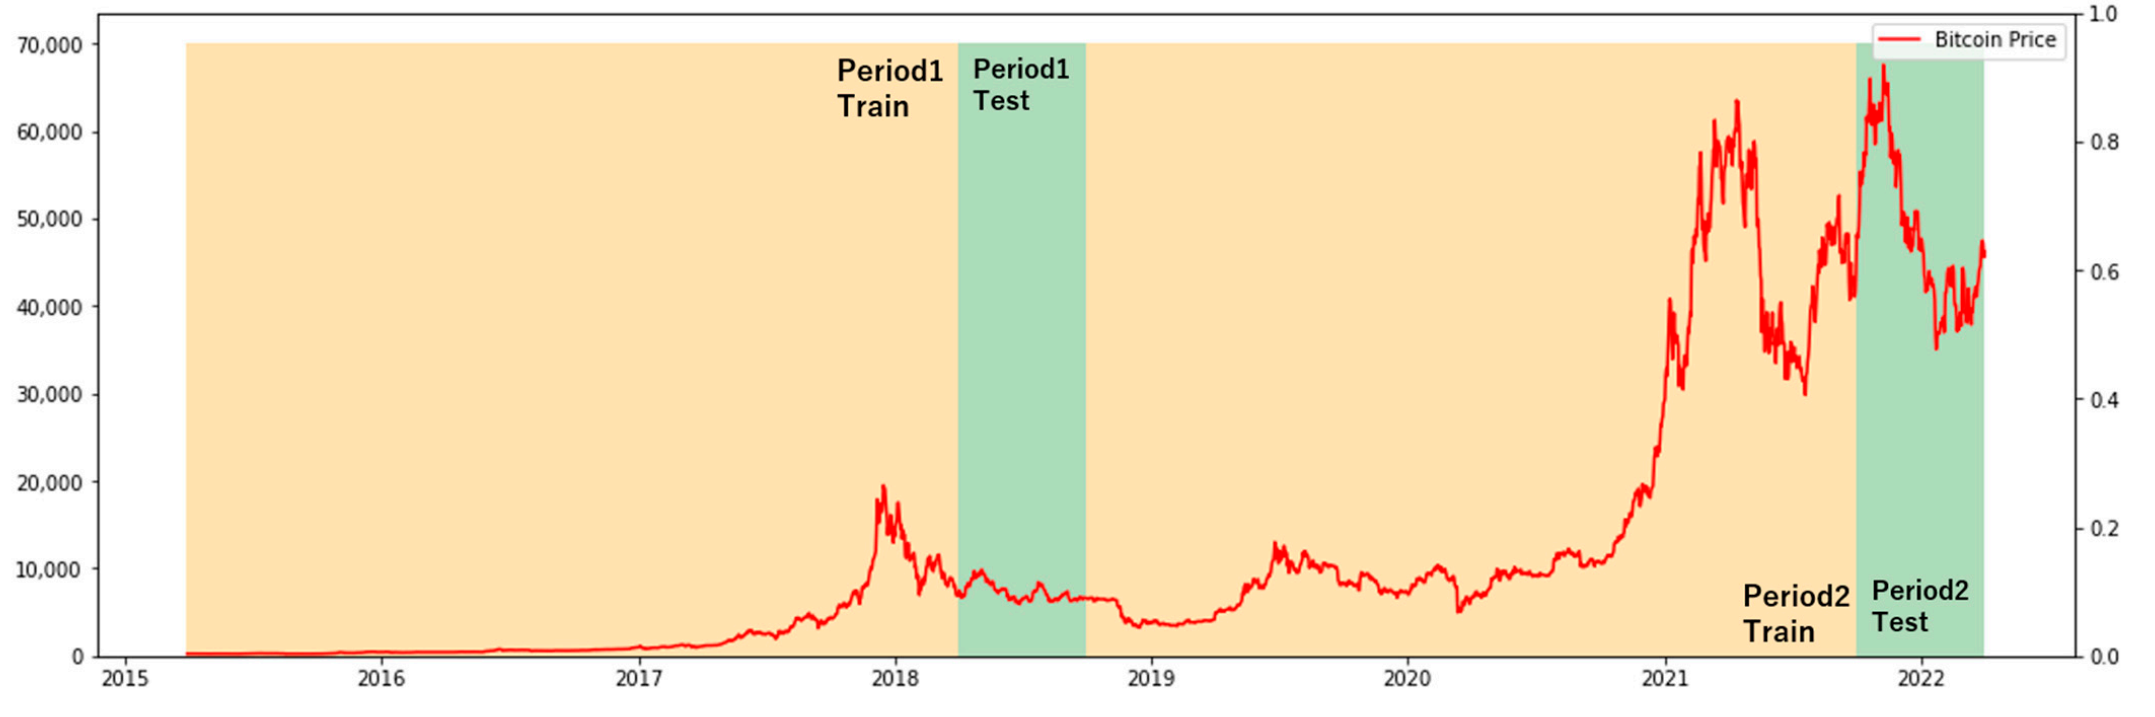
\includegraphics[width=\textwidth, keepaspectratio]{images/Chapter4/divine_dataset.png}
    \caption{Cách chia bộ dữ liệu của tác giả}
    \label{fig:divine_dataset}
\end{figure}


Vì hầu hết những dữ liệu bị thiếu là do những ngày nghỉ cuối tuần, ngày lễ, hoặc thảm họa, nên tác giả cũng đã đề xuất việc \textbf{forward-filling} cho bộ dữ liệu. Forward-filling là một kỹ thuật trong xử lý dữ liệu bị thiếu, nó sẽ điền giá trị bị thiếu bằng giá trị gần nhất mà không bị thiếu. Ở đây tức là giá trị của ngày hôm trước.

Với hầu hết các mô hình học sâu hiện tại, việc \textbf{chuẩn hóa dữ liệu} là điều cần thiết vì điều này sẽ khiến gradient hội hiệu quả hơn và giúp gradient hội tụ một cách cân đối. Ví dụ như việc các hàm kích hoạt như $ReLU$ và $sigmoid$ sẽ rất khó hội tụ khi giá trị âm quá lớn (với hàm $ReLU$) hoặc dương quá lớn thì sẽ khiến cho các hàm này rất khó hội tụ khi đã ở miền phẳng..

\subsection{Mô hình của tác giả}
Để tìm ra mô hình tốt nhất, tác giả đã sử dụng \textbf{GridSearchCV} từ gói phần mềm học máy \textbf{scikit-learn} để tìm ra bộ tham số tốt nhất cho cả hai mô hình tác giả đề xuất. 

Với mô hình Hồi quy Rừng ngẫu nhiên (Random Forest), tác giả sử dụng 500 cây quyết định với mỗi cây có độ sâu tối đa là 10. 

Sử dụng phương pháp tương tự, tác giả đề xuất một mô hình \textbf{LSTM} với 9 lớp (bao gồm một lớp output) như sau:

\begin{table}[hbpt]
    \centering
    \begin{tabular}{lll}
    \hline
    Layer & Layers & Parameters \\
    \hline
    Layer\_1 & LSTM\_1 & units: 128 \\
    & & Activation: ReLU \\
    Layer\_2 & Dropout\_1 & 0.2 \\
    Layer\_3 & LSTM\_2 & units: 128 \\
    & & Activation: ReLU \\
    Layer\_4 & Dropout\_2 & 0.3 \\
    Layer\_5 & LSTM\_3 & units: 256 \\
    & & Activation: ReLU \\
    Layer\_6 & Dropout\_3 & 0.4 \\
    Layer\_7 & LSTM\_4 & units: 256 \\
    & & Activation: ReLU \\
    Layer\_8 & Dropout\_4 & 0.5 \\
    Layer\_9 & Dense & units: 1 \\
    \hline
    \end{tabular}
    \caption{Mô hình LSTM được đề xuất}
    \label{tab:nn_architecture}
\end{table}

Activation function ở đây là hàm kích hoạt trạng thái (thông thường sẽ sử dụng hàm $tanh$), còn hàm kích hoạt hồi quy vẫn sẽ được sử dụng là hàm $sigmoid$.
Ngoài ra, một thông số nữa cũng khá quan trọng của các mô hình học sâu đó chính là epoch. Epoch là số lần mà toàn bộ dữ liệu được đưa qua mạng nơ-ron. Mỗi epoch sẽ được chia thành nhiều batch, và mỗi batch sẽ được đưa qua mạng nơ-ron. Ở giai đoạn 1, tác giả đã đề xuất cài đặt số epoch là 250, và giai đoạn 2, tác giả đã đề xuất cài đặt số epoch là 75.

\subsection{Các thang đo đánh giá mô hình}\label{sec: metrics}
Để đánh giá độ chính xác của một mô hình hồi quy, tác giả đã sử dụng các thang đo sau:
\begin{itemize}
    \item \textbf{Root Mean Squared Error (RMSE)}: RMSE là một thang đo đánh giá mức độ chênh lệch giữa giá trị dự đoán và giá trị thực tế. RMSE càng nhỏ thì mô hình càng tốt.
    \begin{equation}
        RMSE = \sqrt{\frac{1}{n}\sum_{i=1}^{n}(y_i - \hat{y}_i)^2}
    \end{equation}
    \item \textbf{Mean Absolute Percentage Error (MAPE)}: MAPE là một thang đo đánh giá mức độ chênh lệch giữa giá trị dự đoán và giá trị thực tế. MAPE càng nhỏ thì mô hình càng tốt.
    \begin{equation}
        MAPE = \frac{1}{n}\sum_{i=1}^{n}\left|\frac{y_i - \hat{y}_i}{y_i}\right|
    \end{equation}
    \item \textbf{Decision Accuracy (DA)}: DA là một thang đo đánh giá mức độ chính xác của mô hình. DA càng cao thì mô hình càng tốt. DA được tính bằng cách so sánh sự tăng hoặc giảm của giá trị dự đoán ngày hôm trước và ngày hôm sau. \textit{Nếu giá trị dự đoán và giá trị thực tế cùng tăng (hoặc cùng giảm) thì mô hình được tính là dự đoán đúng, ngược lại thì mô hình được tính là dự đoán sai.} Công thức tính DA như sau:
    \begin{equation}
        DA = (\frac{1}{n}\sum_{i=1}^{n}a(i)) * 100\%
    \end{equation}
\end{itemize}

Để so sánh kết quả giữa các mô hình, tác giả đã sử những giả thuyết kiểm định sau:
\begin{itemize}
   \item \textbf{Kiểm định Diebold-Mariano (DM)}: Nguyên lý của kiểm định DM có thể tóm tắt đơn giản như sau: cho hai tập chuỗi sai số dự đoán ${\{e'_t\}}^T_{t=1}$ và ${\{e_t\}}^T_{t=1}$, sau đó định nghĩa hàm mất mát $d_t = L(e_t) - L(e'_t)$, trong đó $L(e) = e^2$ là sai số bình phương trung bình (MSE) và $L(e) = |e|$ là sai số tuyệt đối trung bình (MAE).
   \begin{equation}
    DM_t = \frac{\overline{d_t}}{se(d_t)}
   \end{equation}
   \item \textbf{Kiểm định Clark-West}: Kiểm định Clark-West thêm vào thành phần $(e_t - e'_t)^2$ trong hàm mất mát của kiểm định Diebold-Mariano của MSE như sau: $f_t := (e_t)^2 - (e'_t)^2 + (e_t - e'_t)^2$, thành phần này cũng có phân phối tiệm cận $N(0,1)$, và cuối cùng thực hiện kiểm định giả thuyết một đuôi trên thống kê $f_t$
\end{itemize}

\subsection{Tổng quan quy trình thực nghiệm của tác giả}

\begin{figure}[h!]
    \centering
    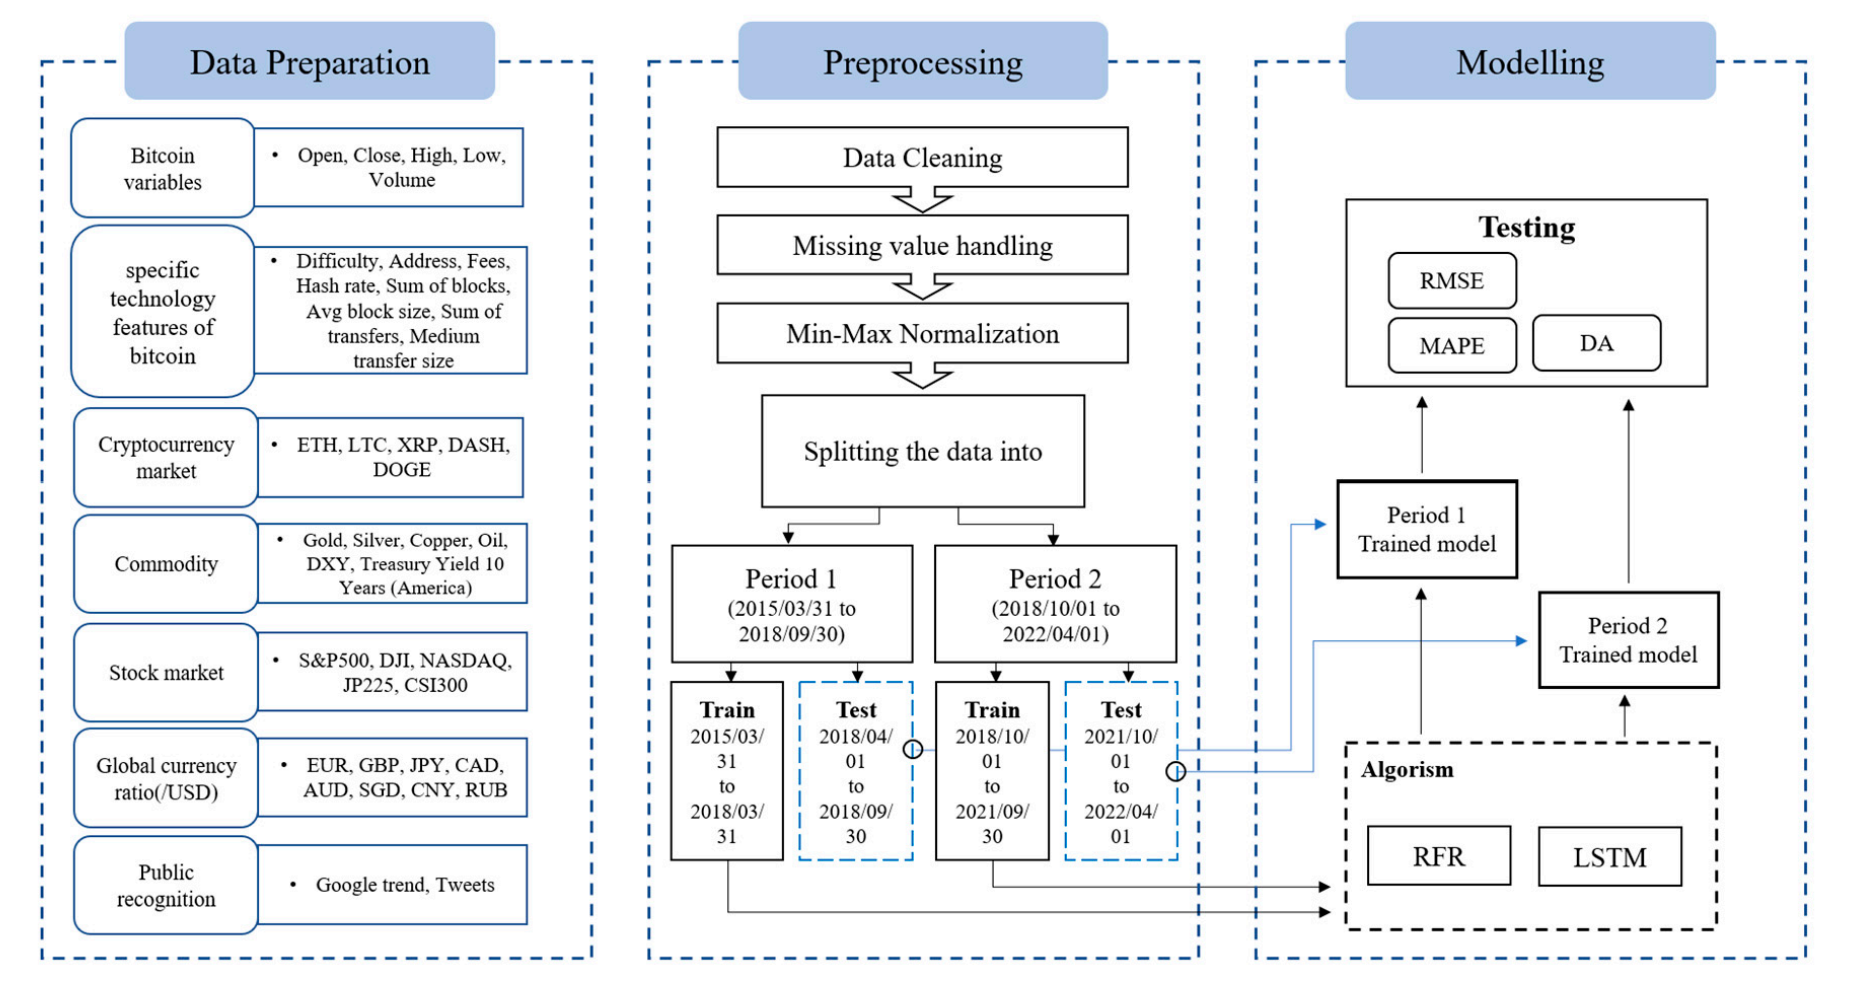
\includegraphics[width=\textwidth, keepaspectratio]{images/Chapter4/process.png}
    \caption{Tổng quan quy trình thực nghiệm tác giả}
    \label{fig:ori_process}
\end{figure}

\begin{table}[h]
    \centering
    \renewcommand{\arraystretch}{1} % Tăng khoảng cách giữa các dòng trong bảng
    \begin{tabular}{|p{7.5cm}|p{7.5cm}|}
        \hline
        \textbf{Ưu điểm} & \textbf{Nhược điểm} \\ \hline
        \begin{itemize}
            \item Forward-filling và chuẩn hóa giúp mô hình hội tụ tốt hơn.
            \item GridSearchCV tối ưu tham số mô hình.
            \item Random Forest với 500 cây giảm overfitting.
            \item LSTM phù hợp với dữ liệu chuỗi thời gian dài.
            \item Dropout giúp giảm overfitting trong LSTM.
            \item Số epoch được điều chỉnh hợp lý cho từng giai đoạn.
        \end{itemize} 
        & 
        \begin{itemize}
            \item Mô hình LSTM yêu cầu tài nguyên tính toán cao.
            \item LSTM có thể overfit nếu dữ liệu huấn luyện không đủ.
            \item Cần điều chỉnh tham số thủ công mất thời gian.
            \item Mô hình phức tạp, khó giải thích kết quả.
            \item Random Forest tính toán lâu với 500 cây.
            \item Cần phần cứng mạnh để huấn luyện nhanh.
        \end{itemize} \\ \hline
    \end{tabular}
    \caption{Ưu điểm và Nhược điểm của thực nghiệm tác giả}
    \label{tab:uudiem_hanche}
\end{table}

\section{Phương pháp cải tiến của sinh viên}
% Nói qua về cấu hình  (siêu tham số tối ưu)  + kết quả chạy (nhớ thêm ảnh kq)  của từng mô hình
% LUU Ý NHO NOI THEM VE CACH CHON va xu ly du lieu feature của từng model
\subsection{XGBoost (Extreme Gradient Boosting)}
\subsection{GRU}
\subsection{Stacking}

\section{So sánh và kết luận}
% Lap bảng so sánh -> Kết luận -> Giải thích tại sao nó tốt hơn ?
% CHÚ Ý so sánh với kết quả của tác giả TRONG BÀI BÁO nêu ra thôi

\input{chapters/chapter6}

\chapter{Phân tích mở rộng \\ Thực nghiệm và so sánh mở rộng}
\section{Vấn đề bài báo gốc} 
\section{Mô hình của tác giả} 
\subsection{LSTM}
\subsection{Random Forest}


\section{Mô hình của sinh viên}
\subsection{GRU}
\subsection{XGBoost}
\subsubsection*{Giới thiệu}
\textit{Boosting} là một trong các kỹ thuật hoc máy kết hợp phổ biến. Bằng cách kết hợp những mô hình yếu lại với nhau - phổ biến nhất là cây quyết định giống như trong thuật toán Random Forest, Boosting cũng đem lại hiệu quả rất tốt. XGBoost là một trong số những mô hình mạnh và đã giành được rất nhiều những thành công và cũng đã có một thời kỳ rất áp đảo trên các cuộc thi trên Kaggle. Ý tưởng tổng quan của kỹ thuật boosting là huấn luyện các mô hình dự đoán một cách tuần tự - các mô hình sau sẽ cố gắng sửa lại những gì còn sai sót của các mô hình từ các bước trước đó.
\subsubsection*{Gradient Boosting}
Với ý tưởng tổng quan là cải thiện dự đoán của các mô hình trước, ta có thể hình dung cơ chế hoạt động của Gradient Boosting là như sau
Ta gọi tập đầu vào là tập $X$, tập đầu ra là $y$. Trước hết ta sẽ tiến hành dự đoán cho cây quyết định thứ nhất. Ở đây ta sẽ sử dụng mô-đun \textit{DecisionTreeRegressor} trong \textit{sci-kit learn}
\begin{verbatim}
    from sklearn.tree import DecisionTreeRegressor
    tree_reg1 = DecisionTreeRegressor()
    tree_reg1.fit(X, y)
\end{verbatim}
Tiếp theo đó, ta sẽ tiếp tục huấn luyện một cây quyết định mới dựa trên lỗi dư thừa (residual error) từ cây quyết định đầu tiên
\begin{verbatim}
    y2 = y - tree_reg1.predict(X)
    tree_reg2 = DecisionTreeRegressor()
    tree_reg2.fit(X, y2)
\end{verbatim}
Tiếp tục lặp lại, như vậy cho đến khi đạt đến một ngưỡng cây nhất định $n$ - một trong những siêu tham số được cài đặt bởi người dùng. Giờ ta đã có một mô hình kết hợp gồm $n$ cây quyết định, và dự đoán của mô hình sẽ được tính bằng tổng dự đoán của các cây
\begin{verbatim}
    trees = [tree_reg1, tree_reg2, ..., tree_regn]
    y_pred = sum(tree.predict(X_test) for tree in trees)
\end{verbatim}
Dưới đây sẽ là đoạn mã giả mô phỏng cách hoạt động của mô hình Gradient Boosting\\

\begin{algorithm}[H]
    \caption{Gradient Boosting với Cây Quyết Định}
    \SetKwFunction{FitTree}{FitTree}
    \SetKwFunction{UpdatePredictions}{UpdatePredictions}
    \SetKwFunction{ComputeResiduals}{ComputeResiduals}
    \SetKwFunction{PredictTest}{PredictTest}
    \SetKwProg{Fn}{Function}{:}{}
    \KwIn{Tập dữ liệu $(X, y)$, số lượng cây $n_{\text{trees}}$, tốc độ học $\alpha$}
    \KwOut{Dự đoán cho tập kiểm tra $y_{\text{test\_pred}}$}
    
    Khởi tạo $\text{trees} \gets []$ (danh sách các cây rỗng)\;
    
    \Fn{\FitTree{$X, y$}}{
        Huấn luyện một DecisionTreeRegressor trên $(X, y)$\;
        \Return cây đã được huấn luyện\;
    }
    
    \textbf{Bước 1: Huấn luyện cây đầu tiên}\;
    $\text{tree}_1 \gets$ \FitTree{$X, y$}\;
    Thêm $\text{tree}_1$ vào $\text{trees}$\;
    $y_{\text{pred}} \gets \text{tree}_1(X)$ (dự đoán ban đầu)\;
    
    \textbf{Bước 2: Huấn luyện các cây tiếp theo}\;
    \For{$i = 2$ đến $n_{\text{trees}}$}{
        Tính sai sót: $r \gets y - y_{\text{pred}}$\;
        $\text{tree}_i \gets$ \FitTree{$X, r$}\;
        Thêm $\text{tree}_i$ vào $\text{trees}$\;
        Cập nhật dự đoán: $y_{\text{pred}} \gets y_{\text{pred}} + \alpha \cdot \text{tree}_i(X)$\;
    }
    
    \textbf{Bước 3: Thực hiện dự đoán trên tập kiểm tra}\;
    $y_{\text{test\_pred}} \gets \sum_{\text{tree} \in \text{trees}} \alpha \cdot \text{tree}(X_{\text{test}})$\;
    
    \Return $y_{\text{test\_pred}}$\;
\end{algorithm}
\subsubsection*{So sánh Gradient Boosting và XGBoost}
Những điểm mạnh và cải tiến của mô hình XGBoost so với Gradient Boosting truyền thống:
\begin{itemize}
    \item \textbf{Điều chuẩn - Regularization:} XGBoost có thêm một số siêu tham số để penalize những mô hình phức tạp thông qua điều chuẩn L1 và L2 giúp tránh việc overfitting.
    \item \textbf{Kiểm soát dữ liệu thiếu hoặc thưa:} Trong một số trường hợp, dữ liệu có thể bị thiếu, hoặc các kỹ thuật tiền xử lý dữ liệu đôi khi có thể làm dữ liệu bị thưa. Tuy nhiên, XGBoost đã được tích hợp sẵn sàng thuật toán chia nhánh có kiểm soát dữ liệu thưa.
    \item \textbf{Thuật toán Weighted Quantile Sketch:} Hầu hết các thuật toán cây hiện có đều chỉ tìm được điểm chia khi các điểm dữ liệu có trọng số bằng nhau (sử dụng thuật toán quantile sketch thông thường). Tuy nhiên, chúng không được thiết kế để xử lý dữ liệu có trọng số. XGBoost có một thuật toán phân tán weighted quantile sketch, cho phép xử lý hiệu quả dữ liệu có trọng số không đồng đều.
    \item \textbf{Cấu trúc khối để học song song (Block Structure for Parallel Learning):} Để tính toán nhanh hơn, XGBoost có thể sử dụng nhiều lõi (cores) trên CPU. Điều này khả thi nhờ vào cấu trúc khối trong thiết kế hệ thống. Dữ liệu được sắp xếp và lưu trữ trong các đơn vị bộ nhớ gọi là blocks. Khác với các thuật toán khác, cách tiếp cận này cho phép tái sử dụng cấu trúc dữ liệu đã lưu trữ thay vì tính toán lại qua mỗi lần lặp. Tính năng này đặc biệt hữu ích cho các bước như tìm điểm chia (split finding) và lấy mẫu cột (column sub-sampling).
    \item \textbf{Nhận thức bộ nhớ đệm (Cache Awareness):} Trong học máy với XGBoost, ngôn ngữ Scala yêu cầu truy cập bộ nhớ không liên tục để lấy các thống kê gradient theo chỉ mục hàng. Do đó, Tianqi Chen đã thiết kế XGBoost để tối ưu hóa việc sử dụng phần cứng. Quá trình tối ưu này được thực hiện bằng cách cấp phát các bộ đệm nội bộ (internal buffers) trong từng luồng xử lý, nơi mà workflow có thể lưu trữ thống kê gradient. Nhờ đó, các cây được xây dựng song song một cách hiệu quả hơn, đặc biệt khi tận dụng ngôn ngữ Julia và Java.
    \item \textbf{Tính toán ngoài bộ nhớ (Out-of-Core Computing):} Tính năng này tối ưu hóa không gian đĩa có sẵn và tận dụng tối đa khi xử lý các tập dữ liệu lớn không thể vừa trong bộ nhớ RAM.
\end{itemize}

\subsection{Stacking}
\section{So sánh và kết luận}
\chapter{Ứng dụng mở rộng vào thực tế}
\section{Ứng dụng vào thực tế} % Kiẹt viet
% dự đoán cho giá BTC 2023 -2024
\section{Mô hình của sinh viên} 
% Nhớ nói là AE CHẠY TRÊN TOÀN BỘ DỮ LIỆU GỐC tác giả -> Dùng mô hình -> DỰ ĐOÁN CHO GIÁ BTC 2023-2024
% Cấu hình của mô hình (siêu tham số tối ưu mới)  +  Kết quả chạy (nhớ thêm ảnh kq) 
\subsection{GRU}
\subsection{Stacking}
\subsection{GRU-XGBoost} %Nho noi them co so ly thuyet
\subsection{LSTM-GRU} %Nho noi them co so ly thuyet

\section{Kết quả và kết luận}
%Tổng hợp lại toàn bộ kết quả -> kết luận ?
\singlespacing

\clearpage
\bibliography{refs}
% \addcontentsline{toc}{chapter}{References}
\addcontentsline{toc}{chapter}{Tài liệu tham khảo}
\bibliographystyle{unsrt}


% \renewcommand{\appendixname}{Phụ lục} % Change "Appendices" to "Phụ lục"
% \addcontentsline{toc}{chapter}{Phụ lục} % Add "Phụ lục" to the table of contents
% \chapter*{This is title of appendix A}
% \addcontentsline{toc}{chapter}{Phụ lục A}
% \blindmathpaper
% \chapter*{This is title of appendix B}
% \addcontentsline{toc}{chapter}{Phụ lục B}
% \blindmathpaper

\end{document}
